% !TEX program = xelatex
% =============================================================================
%  OceanSwarm 开发文档（中文，XeLaTeX + ctex）
%  编译：xelatex OceanSwarm-dev-doc.tex （连续两次以生成目录）
% =============================================================================
\documentclass[UTF8, a4paper, 11pt]{ctexart}

\usepackage{geometry}
\geometry{left=2.4cm, right=2.4cm, top=2.6cm, bottom=2.5cm}
\usepackage{graphicx}
\usepackage{xcolor}
\usepackage{colortbl}
\usepackage{amsmath}
\usepackage{amssymb}
\usepackage{booktabs}
\usepackage{array}
\usepackage{multirow}
\usepackage{caption}
\usepackage{subcaption}
\usepackage{float}
\usepackage{longtable}
\usepackage{fancyhdr}
\usepackage{tikz}
\usetikzlibrary{arrows.meta, positioning, shapes.geometric, calc}
\usepackage{listings}
\usepackage{hyperref}

\definecolor{themeblue}{HTML}{1C5A96}
\definecolor{themecoral}{HTML}{E08F96}
\definecolor{themecyan}{HTML}{2BC8C0}
\definecolor{themegray}{HTML}{4A5A66}
\definecolor{codebg}{HTML}{F4F7FA}
\definecolor{codeframe}{HTML}{C8D6E2}
\definecolor{linkcolor}{HTML}{1565A8}
\definecolor{palpearl}{HTML}{F4F6F4}
\definecolor{palnavy}{HTML}{173A56}
\definecolor{palsilver}{HTML}{C5D0D6}
\definecolor{palcyan}{HTML}{4CEFE0}
\definecolor{palorange}{HTML}{FF8C2E}
\definecolor{palhull}{HTML}{073A51}
\definecolor{palmid}{HTML}{0E617E}
\definecolor{pallight}{HTML}{1E94A1}
\definecolor{palcrest}{HTML}{C8F5E8}
\definecolor{palrock}{HTML}{7A8488}
\definecolor{palgold}{HTML}{FFD27A}
\definecolor{palshallow}{HTML}{3ECFBD}
\definecolor{palhaze}{HTML}{B7D6E5}

\hypersetup{
  colorlinks=true,
  linkcolor=themeblue,
  citecolor=themeblue,
  urlcolor=linkcolor,
  pdftitle={OceanSwarm 未来智能无人艇集群协同巡航海域开发文档},
  pdfauthor={朱华天},
  pdfsubject={Three.js 大型三维海洋场景},
  pdfkeywords={Three.js, Vite, USV, 海洋场景, 程序化生成, HDR 天空, 法线贴图, 三渲二}
}

\captionsetup{font=small, labelsep=quad}
\captionsetup[subfigure]{font=small}

\pagestyle{fancy}
\fancyhf{}
\fancyhead[L]{\small\color{themegray}OceanSwarm 开发文档}
\fancyhead[R]{\small\color{themegray}\thepage}
\renewcommand{\headrulewidth}{0.3pt}
\renewcommand{\headrule}{\hbox to\headwidth{\color{codeframe}\leaders\hrule height \headrulewidth\hfill}}

\lstdefinestyle{code}{
  backgroundcolor=\color{codebg},
  frame=single,
  rulecolor=\color{codeframe},
  basicstyle=\ttfamily\footnotesize,
  keywordstyle=\color{themeblue}\bfseries,
  commentstyle=\color{themegray}\itshape,
  stringstyle=\color{themecoral!80!black},
  numbers=left,
  numberstyle=\tiny\color{themegray},
  numbersep=7pt,
  breaklines=true,
  columns=fullflexible,
  keepspaces=true,
  showstringspaces=false,
  tabsize=2,
  aboveskip=8pt,
  belowskip=8pt,
  xleftmargin=1.4em,
  framexleftmargin=1.2em
}
\lstset{style=code}

\newcommand{\file}[1]{\texttt{#1}}
\newcommand{\repolink}{\href{https://github.com/ZHT1235456/OceanSwarm}{\texttt{https://github.com/ZHT1235456/OceanSwarm}}}

% -----------------------------------------------------------------------------
\begin{document}

% ============================ 封面 ==========================================
\begin{titlepage}
\centering
\vspace*{1.2cm}
{\color{themeblue}\rule{\linewidth}{1.2pt}}\\[0.9cm]
{\huge\bfseries\color{themeblue} 未来智能无人艇集群\\[0.35cm]协同巡航海域}\\[0.9cm]
{\LARGE 基于 Three.js 的大型三维海洋场景\\[0.3cm]开发文档}\\[0.9cm]
{\color{themeblue}\rule{\linewidth}{1.2pt}}\\[1.6cm]

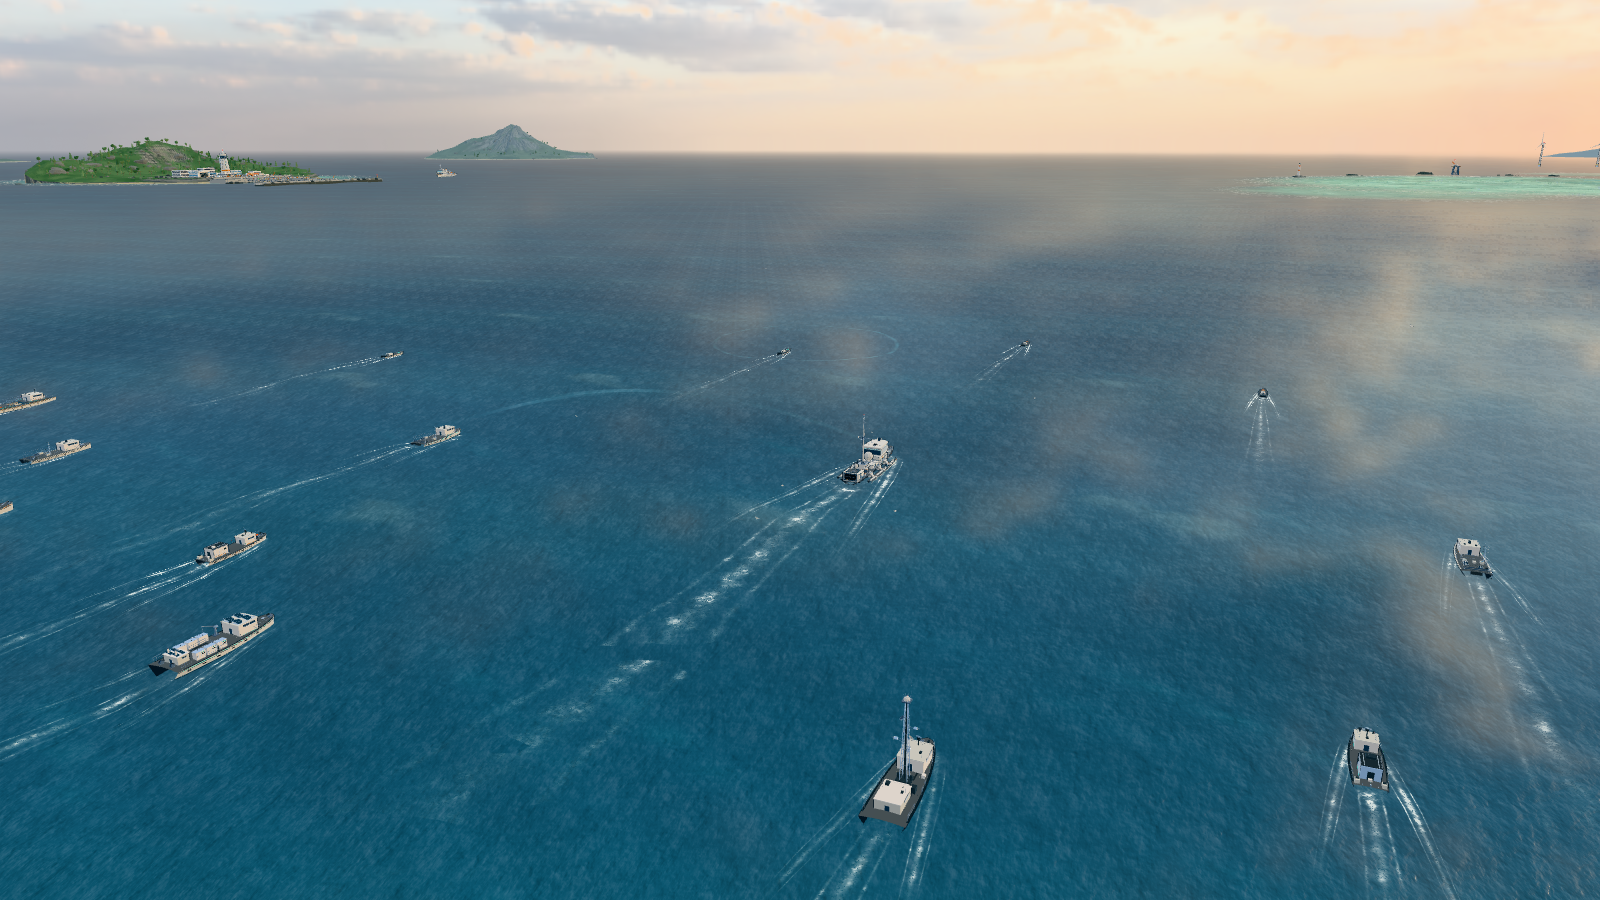
\includegraphics[width=0.92\linewidth]{figures/fig-00-hero.png}\\[1.1cm]

{\large
\begin{tabular}{rl}
\textbf{作者：} & 朱华天 \\[0.35em]
\textbf{模型：} & DeepSeek V4.1 Flash 1017 \\[0.35em]
\textbf{日期：} & 2026 年 10 月 22 日 \\[0.35em]
\textbf{项目仓库：} & \repolink \\
\end{tabular}}
\vfill
{\small\color{themegray}版本 v1.2 \quad|\quad Three.js 0.186 \quad|\quad Vite 7 \quad|\quad 程序化场景 + 本地 HDR 天空 / 水面法线贴图}
\end{titlepage}

% ============================ 摘要 ==========================================
\pagenumbering{Roman}
\begin{abstract}
\noindent
本文档完整记录“OceanSwarm —— 未来智能无人艇集群协同巡航海域”这一大型三维海洋场景的设计与实现。项目使用 Three.js 与 Vite 构建：外部素材只有两张随仓库分发的本地贴图——CC0 许可的 2K HDR 天空全景（Poly Haven “Kloppenheim 06 (Pure Sky)”）与 three.js 官方示例水面法线贴图（MIT）；船体、海岛、珊瑚礁、波浪、尾迹与光效全部以程序化几何与着色器实时生成。场景是一片数公里尺度的开放海域：17 艘不同任务的智能无人水面艇（含一艘 30 米三体无人指挥旗舰）沿宽阔圆弧航线协同巡航，海面上分布着连续的历史轨迹尾迹、破浪泡沫与克制的青蓝色通信光效；远景由岩石海岛、海上无人系统试验基地、保障母船、珊瑚礁潟湖、航标灯塔与风电场共同构成层次分明的海天空间，天空由同一张 HDR 全景提供真实方向的积云、深蓝天顶与低角度暖阳，海面则由程序化波形叠加三层照片法线微细节，配合暗水体基底与 HDR 环境反射。文档依次介绍项目目标、运行方式、总体架构、程序化海洋与 HDR 天空、无人艇建模、编队动力学、尾迹与光效、海域环境、美术与光照方案、性能与质量验证，并给出完整的参数表、代码摘录与实机截图。项目可直接通过 \file{npm run dev} 运行，开发服务器不发起任何外部网络请求；生产构建 JavaScript 约 867~KB（gzip 247~KB），加上本地 HDR 4.43~MB 与水面法线 249~KB 后 \file{dist/} 约 5.55~MB。实测约 537 个绘制调用、78.5 万个三角形、5 张纹理，控制台零错误、界面零 UI，HDR 全景与水面法线贴图请求全部为本地 HTTP 200。

\vspace{0.6em}
\noindent\textbf{关键词：} Three.js；Vite；无人水面艇（USV）；程序化建模；海洋着色器；三渲二；实时渲染
\end{abstract}

\newpage
\tableofcontents
\newpage

% ============================ 正文 ==========================================
\pagenumbering{arabic}
\setcounter{page}{1}

% -----------------------------------------------------------------------------
\section{项目概述}

\subsection{背景与目标}

本项目以“未来海洋无人系统试验海域”为主题，目标是制作一个可以直接在浏览器中自由探索的大型三维场景：观众打开页面后，应立刻看到辽阔连续的蓝色海洋、清晰的海天交界线、一支正在协同巡航的无人艇集群，以及由海岛、海上基地、珊瑚礁与远方云层构成的完整海洋世界。

与常见的游戏 Demo 不同，本项目在约束上非常明确：

\begin{itemize}
  \item \textbf{无界面}：画面中不允许出现任何 UI 面板、按钮、文字说明、坐标轴、调试信息或浏览器界面元素，打开即是完整场景；
  \item \textbf{资源自包含与离线运行}：外部美术资源只有两张随仓库分发的本地贴图——CC0 许可的 2K HDR 天空全景，以及 three.js 官方示例水面法线贴图（MIT）；船体、地形、波形、泡沫、尾迹与光效均由程序化几何与着色器实时生成，不使用任何外部模型，运行时不访问网络，可完全离线运行；
  \item \textbf{真实尺度感}：以米为单位建模，海域半径约 26~km，无人艇 6--30~m，海岛 300--1250~m，海上指挥塔约 62~m，通过近大远小、空气透视与雾效形成强烈纵深感；
  \item \textbf{优先保证大效果}：在性能预算内优先保证海洋连续性、编队完整度、旗舰精细度、尾迹与海天氛围，其次才是细小的装饰。
\end{itemize}

\subsection{最终成果}

最终场景包含：

\begin{itemize}
  \item 一片半径 26~km 的海面：CPU/GPU 共用同一套 7 组方向波，叠加三层拉伸漂移的照片法线微细节（近景毛细波、中景细浪、远景风斑），暗色基底与 HDR 环境反射共同塑形；海面网格随相机移动，菲涅尔反射与远处地平线雾逐方向采样同一张 HDR 全景，与天空穹顶无缝衔接；
  \item 17 艘无人艇：1 艘 30~m 三体旗舰、5 艘高速侦察艇、3 艘环境监测艇、2 艘双体测绘艇、2 艘多用途巡逻艇，以及通信中继、能源保障各 1--2 艘和 1 艘无人救援艇；
  \item 完整的编队行为：旗舰沿半径约 1.6~km 的大圆弧缓慢转向，各艇以指数弹簧保持阵位并带自然摆动，侦察艇周期性向外展开，所有船体随浪升沉、纵摇与横摇；
  \item 每艘船独立的轨迹尾迹、船首 V 形破浪、船侧泡沫线、尾流泡沫，共 17 套动态泡沫网格；
  \item 左后方海岛上的无人系统试验基地（62~m 指挥塔、模块化科研建筑、封闭连廊、三组桩基码头、集装箱场、防波堤）、120~m 保障母船；右前方浅海珊瑚礁潟湖（海底沙脊、498 组珊瑚、海草、三个鱼群、焦散光斑）；中远景的三座海岛、航标浮标阵列、灯塔、自升式观测平台与五台海上风机；
  \item 由本地 2K HDR 全景驱动的天空大气：金色逆光积云、散布积云与深蓝天顶，方位角 $40.7^\circ$、仰角 $4.7^\circ$ 的低角度暖阳，太阳一侧暖金、背光一侧冷蓝的地平线；同一全景还提供海面反射、距离雾与金属/玻璃的 IBL 环境光；少量海鸥与克制的青蓝色协同可视化光效。
\end{itemize}

\begin{figure}[H]
  \centering
  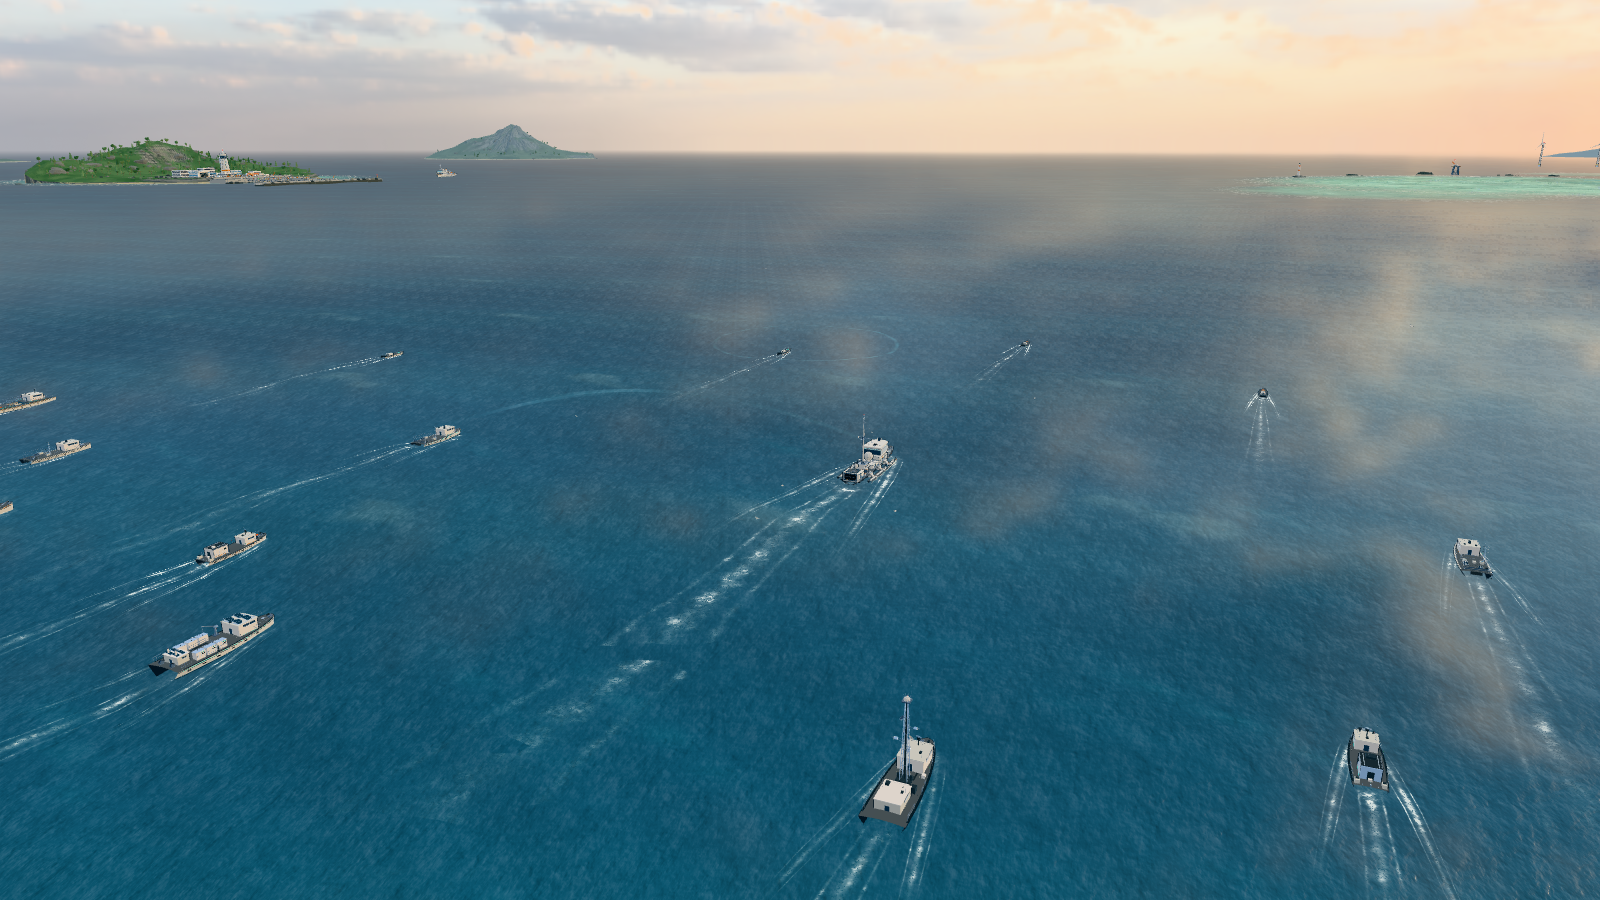
\includegraphics[width=\linewidth]{figures/fig-00-hero.png}
  \caption{初始镜头下的完整场景：连续海面、无人艇编队、白色尾迹、左侧研究海岛与远方海天交界线。}
  \label{fig:hero}
\end{figure}

\subsection{需求与实现对照}

表~\ref{tab:req-map} 概括了需求要点与对应的实现手段。

\begin{table}[H]
\centering
\caption{核心需求与实现方式对照}
\label{tab:req-map}
\small
\begin{tabular}{@{}p{0.30\linewidth}p{0.62\linewidth}@{}}
\toprule
\textbf{需求要点} & \textbf{实现方式} \\
\midrule
无 UI、打开即场景 & 全屏 canvas，无任何 DOM 覆盖层；相机与场景由 \file{src/main.js} 直接装配 \\
广阔连续海洋 & 26~km 半径径向网格 + 相机跟随 + 距离波衰减 + 方向相关雾色 + 三层照片法线细节 \\
清晰海天交界线 & 海面距离雾逐方向采样同一 HDR 全景的地平线颜色（\texttt{skyRadiance()}），两边颜色一致 \\
15--20 艘集群 & 17 艘：1 旗舰 + 16 艘 7 个类别，程序化参数化船体与模块化设备 \\
精细中央旗舰 & 30~m 三体结构、13 个材质批次合批 + 描边、3 组动态设备、61k 三角形 \\
白色航行尾迹 & 每船历史轨迹带 + 船首 V 形臂 + 泡沫项圈 + 尾流，自定义泡沫着色器 \\
岛屿与海上基地 & 噪声高度场海岛、分层岩壁、程序化建筑群、桩基码头与地形高度采样贴合 \\
天空阳光云层 & 本地 2K HDR 全景（CC0）等距圆柱穹顶 + 方位/仰角对齐的太阳 + HDR PMREM 环境反射（缺失时回退程序化天空） \\
水面微细节 & 本地 1024$^2$ 照片法线贴图三层拉伸漂移（毛细波 / 细浪 / 风斑）+ 低角度太阳微明暗 + 暗水体基底 \\
科技光效克制 & 6 条低透明度通信弧、扫描环、测绘扇形光束，均无文字与面板 \\
性能与尺度 & 合批 + InstancedMesh + 关闭实时阴影 + 像素比上限，约 537 次绘制、78.5 万三角形 \\
\bottomrule
\end{tabular}
\end{table}

% -----------------------------------------------------------------------------
\section{运行与操作}

\subsection{环境与命令}

项目使用 Node.js（建议 $\ge$ 18）与 npm 管理依赖，核心依赖为 \file{three@0.186} 与 \file{vite@7}。两张本地素材已随仓库提供、无需任何额外下载：天空 HDR 全景（4\,434\,394 字节）与水面法线贴图（248\,813 字节）。Vite 从应用自身的 base URL 以同源方式提供，运行时不访问网络；若 HDR 缺失或解码失败，\file{main.js} 记录 \texttt{console.error} 并回退到程序化天空，若水面法线缺失则回退到程序化涟漪。

生产构建在 \file{vite.config.js} 中设置 \texttt{build.target = 'es2022'}：\file{src/main.js} 用顶层 \texttt{await} 并行预加载 HDR 全景与水面法线贴图（使首帧即具备完整大气与水面细节），而顶层 await 需要 es2022 目标（Chrome/Edge $\ge$ 94、Firefox $\ge$ 93、Safari $\ge$ 15.4）。构建产物 \file{dist/} 合计约 5.55~MB：JavaScript 866.5~KB（gzip 246.6~KB）+ HDR 资源 4.43~MB + 水面法线 249~KB。

\begin{lstlisting}[language=bash, caption={安装与运行命令}, label={lst:run}]
npm install
npm run dev      # 开发服务器 http://127.0.0.1:5179
npm run build    # 生产构建，输出到 dist/
npm run preview  # 预览生产构建
\end{lstlisting}

\subsection{交互方式}

场景基于 \texttt{OrbitControls} 实现第三人称自由观察，并额外加入“编队跟随”平移：每帧相机与观察目标同时叠加编队质心位移，从而在编队持续巡航时保持构图稳定。

\begin{itemize}
  \item \textbf{左键拖拽}：围绕观察目标旋转，带阻尼；
  \item \textbf{滚轮}：平滑缩放，距离限制 16--4200~m；
  \item \textbf{右键拖拽}：沿水平面平移观察；
  \item \textbf{视角限制}：极角限制 $[0.13, 1.505]$~rad，避免镜头穿入水下；相机始终位于水面以上。
\end{itemize}

初始镜头位于编队后方偏右的中高空（相对编队坐标系：后退 225~m、上升 72~m、右移 98~m，视场角 47$^\circ$），俯视约 16$^\circ$，画面中同时呈现旗舰、前方侦察艇、两翼协同艇、后方保障艇、尾迹与海天交界线。

\subsection{开发用取景预设}

为便于开发与质量验证，\file{src/main.js} 内置了一组隐藏的相机预设（不出现在界面中），可通过 \file{?view=} 查询参数或调试钩子切换，见表~\ref{tab:views}。

\begin{table}[H]
\centering
\caption{开发取景预设（不可见于画面）}
\label{tab:views}
\small
\begin{tabular}{@{}lll@{}}
\toprule
\textbf{预设} & \textbf{取景内容} & \textbf{用途} \\
\midrule
\file{default} & 编队后上方全景，含海天交界线 & 首屏与整体构图 \\
\file{low} & 水面以上约 5~m，跟随旗舰前进方向 & 破浪、尾迹、海面低角度 \\
\file{bow} & 旗舰船首左前方约 45~m & 船首、球鼻、设备细节 \\
\file{side} & 旗舰右舷侧向近景 & 船体侧面、灯带、护舷 \\
\file{fleet} & 高高拉起 235~m，回看整个编队 & 编队秩序与尾迹布局 \\
\file{top} & 编队正上方约 780~m & 队形、航迹、海洋纹理 \\
\file{base} & 试验基地、码头与母船 & 远景设施验证 \\
\file{reef} & 珊瑚礁潟湖俯视 & 浅水与生态验证 \\
\bottomrule
\end{tabular}
\end{table}

\begin{figure}[H]
  \centering
  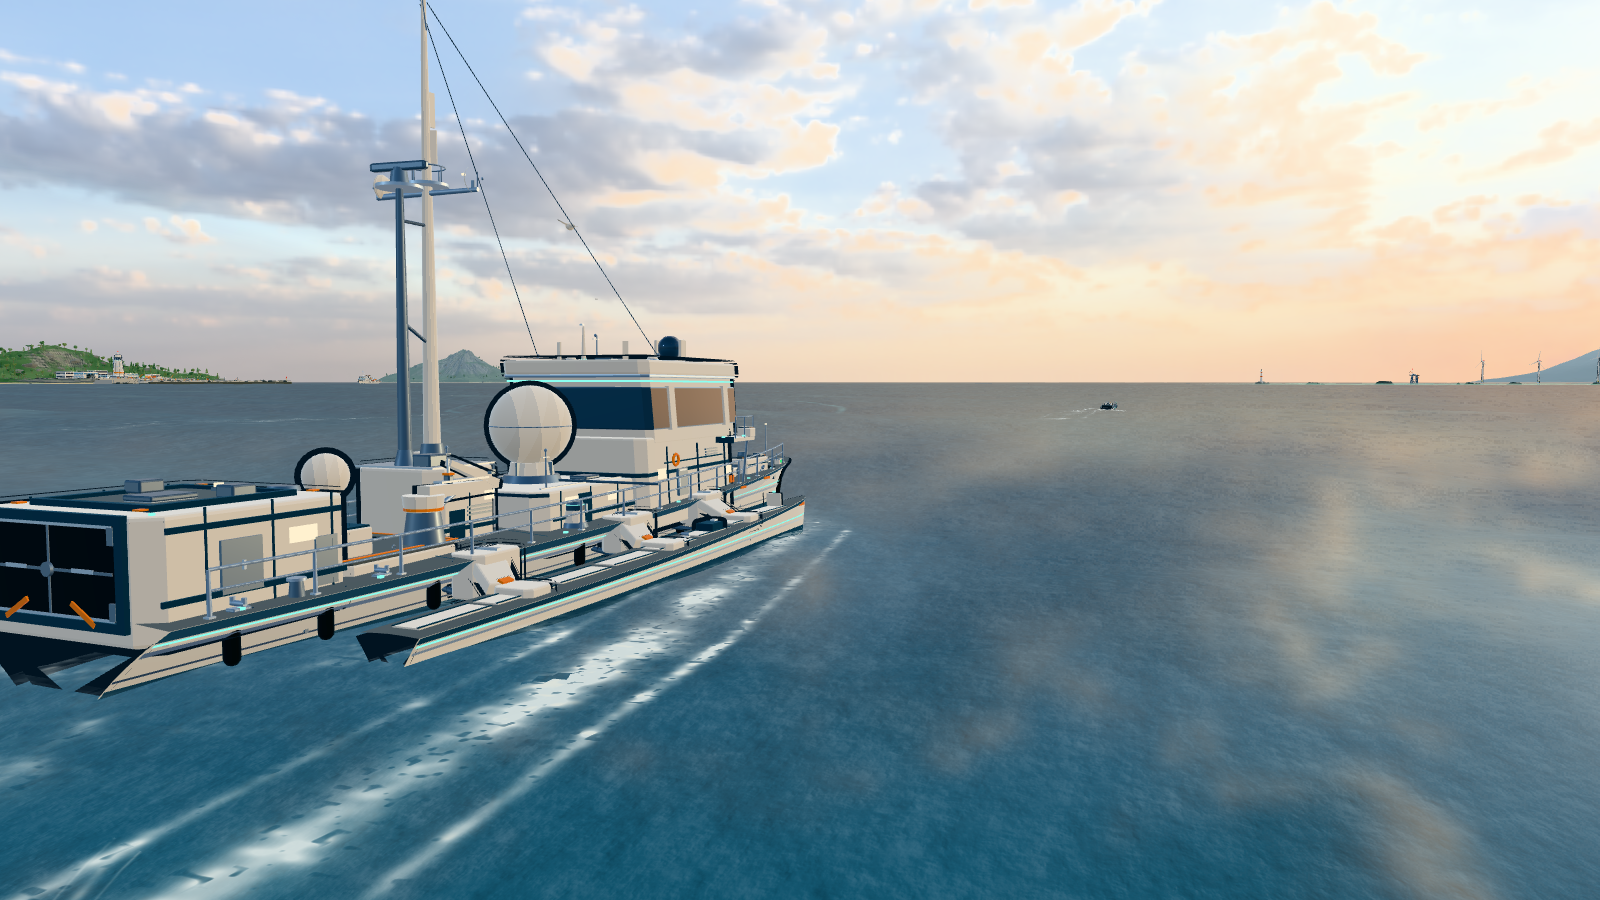
\includegraphics[width=0.95\linewidth]{figures/fig-01-low-angle.png}
  \caption{水面低角度视角：旗舰舷侧、泡沫水线与落日海面。}
  \label{fig:low}
\end{figure}

% -----------------------------------------------------------------------------
\section{总体架构}

\subsection{模块划分}

代码按“配置—核心—系统—对象”四层组织（图~\ref{fig:arch}）。\file{config.js} 集中管理调色板、世界布局、编队名册、相机与光照参数，是全部模块共享的单一事实来源；\file{core/} 提供与具体实体无关的通用能力（几何工具、HDR 全景与水面法线加载、材质库、波场、海面、天空）；\file{systems/} 实现编队运动学；\file{objects/} 按“船—环境—特效”三类组织程序化模型；\file{main.js} 负责装配、相机、渲染循环与调试钩子。

\begin{figure}[H]
\centering
\begin{tikzpicture}[
  font=\footnotesize,
  cfg/.style={draw=themecoral!80, fill=themecoral!12, rounded corners=2pt, align=center, inner sep=4pt},
  box/.style={draw=themeblue!55, fill=themeblue!7, rounded corners=2pt, align=center, inner sep=4pt},
  core/.style={draw=themecyan!80, fill=themecyan!10, rounded corners=2pt, align=left, inner sep=4pt},
  obj/.style={draw=themegray!55, fill=themegray!8, rounded corners=2pt, align=left, inner sep=4pt},
  arr/.style={-{Stealth[length=2.2mm]}, draw=themegray, line width=0.6pt}
]
\node[cfg] (cfg) at (5.2,3.5) {\file{config.js}：调色板 / 世界布局 / 编队名册 / 相机与光照参数};
\node[box] (main) at (5.2,2.35) {\file{main.js}：场景装配、渲染循环、相机跟随、调试钩子};

\node[core, anchor=north, text width=6.0cm] (core) at (0,0.55) {\textbf{core/}：基础能力\\
  \file{geo.js} / \file{hdri.js}：几何 + HDR\\
  \file{water-normal.js}：水面法线\\
  \file{materials.js}：材质 + PMREM\\
  \file{waves.js}：共享波场\\
  \file{ocean.js} / \file{sky.js}：海面 + 天空};

\node[box, anchor=north, text width=2.9cm, align=left] (sys) at (5.1,0.55) {\textbf{systems/}：编队\\
  \file{formation.js}\\ 航线 / 阵位 / 随浪姿态};

\node[obj, anchor=north, text width=3.5cm] (obj) at (9.9,0.55) {\textbf{objects/}：场景实体\\
  \file{ships/}：旗舰与 7 类艇型\\
  \file{world/}：海岛·珊瑚礁·基地·母船·航标\\
  \file{effects/}：尾迹·通信弧·海鸥};

\draw[arr] (cfg) -- (main);
\draw[arr] (main.south) -- (core.north);
\draw[arr] (main.south) -- (sys.north);
\draw[arr] (main.south) -- (obj.north);
\end{tikzpicture}
\caption{项目模块架构：配置层、核心能力层、系统层与对象层。}
\label{fig:arch}
\end{figure}

\subsection{帧循环与数据流}

每帧的计算顺序经过刻意安排，保证“先运动、后接触效果、再环境、最后渲染”（图~\ref{fig:loop}）。特别是尾迹系统需要读取船体最新的世界矩阵，因此必须在队形与船体矩阵更新之后进行（即 \file{fleet.update()} 与矩阵更新之后）。

在进入渲染循环之前，\file{main.js} 用 \texttt{Promise.all} 并行 \texttt{await} 本地 HDR 全景（含 PMREM 环境图）与水面法线贴图，因此首帧就具备一致的天空、海面反射、环境光照与水面细节；任一素材加载失败则返回空值继续，由着色器回退到程序化天空 / 程序化涟漪。

\begin{figure}[H]
\centering
\begin{tikzpicture}[
  font=\small,
  flowstep/.style={draw=themeblue!55, fill=themeblue!6, rounded corners=2pt, align=left, inner sep=4pt, minimum width=8.2cm, minimum height=0.66cm},
  arr/.style={-{Stealth[length=2.2mm]}, draw=themegray, line width=0.6pt}
]
\node[flowstep] (s1) {\textbf{1.} 计算帧间隔 $dt$（上限 0.1~s），累计模拟时间 $t$};
\node[flowstep, below=0.16cm of s1] (s2) {\textbf{2.} \file{fleet.update(dt)}：航路推进、阵位跟随、四点随浪姿态、船内设备动画};
\node[flowstep, below=0.16cm of s2] (s3) {\textbf{3.} 相机与观察目标同时平移编队质心位移，\texttt{controls.update()} 应用阻尼};
\node[flowstep, below=0.16cm of s3] (s4) {\textbf{4.} \file{scene.updateMatrixWorld()}，随后更新尾迹 / 通信光效 / 海鸥};
\node[flowstep, below=0.16cm of s4] (s5) {\textbf{5.} 更新海岛、珊瑚礁、基地、母船、航标等环境动画};
\node[flowstep, below=0.16cm of s5] (s6) {\textbf{6.} 更新海面（跟随相机）与天空（跟随相机），\file{renderer.render()}};
\foreach \a/\b in {s1/s2, s2/s3, s3/s4, s4/s5, s5/s6} \draw[arr] (\a) -- (\b);
\end{tikzpicture}
\caption{每帧数据流。}
\label{fig:loop}
\end{figure}

\subsection{代码结构与规模}

项目共 21 个 JavaScript 源文件，约 14\,000 行（不含依赖）。表~\ref{tab:files} 列出主要文件及其职责。

\begin{table}[H]
\centering
\caption{主要源文件与职责}
\label{tab:files}
\small
\begin{tabular}{@{}p{0.375\linewidth}r p{0.43\linewidth}@{}}
\toprule
\textbf{文件} & \textbf{行数} & \textbf{职责} \\
\midrule
\file{src/config.js} & 261 & 调色板、世界布局、编队名册、相机/光照/雾参数、HDR 与水法线路径 \\
\file{src/main.js} & 425 & HDR 与水法线预加载、渲染器、相机、灯光、模块装配、帧循环、调试钩子 \\
\file{src/core/geo.js} & 625 & 参数化船体、几何工具集、Builder 合批与描边 \\
\file{src/core/hdri.js} & 56 & 本地 HDR 全景加载（HDRLoader + PMREM 环境图） \\
\file{src/core/materials.js} & 290 & 卡通材质库、边缘光、HDR PMREM 环境反射（含回退） \\
\file{src/core/waves.js} & 83 & 7 组方向波、CPU 采样器、GLSL 波场代码 \\
\file{src/core/water-normal.js} & 40 & 水面法线贴图加载（TextureLoader、NoColorSpace/RepeatWrapping/mipmap） \\
\file{src/core/ocean.js} & 453 & 径向海面网格、海洋着色器、三层法线细节、HDR 反射与逐方向地平线雾 \\
\file{src/core/sky.js} & 181 & HDR 天空穹顶、等距圆柱采样、程序化回退 \\
\file{src/systems/formation.js} & 208 & 航线、阵位保持、随浪升沉/纵摇/横摇 \\
\file{src/objects/ships/flagship.js} & 1368 & 30~m 三体旗舰程序化模型与设备动画 \\
\file{src/objects/ships/fleet-types.js} & 2049 & 7 类无人艇、21 种变体装配 \\
\file{src/objects/world/islands.js} & 1359 & 海岛高度场、岩壁、植被、拍岸浪 \\
\file{src/objects/world/reef.js} & 1129 & 珊瑚礁海底、珊瑚、海草、鱼群、焦散 \\
\file{src/objects/world/base.js} & 1518 & 试验基地、码头、防波堤、建筑群 \\
\file{src/objects/world/mothership.js} & 795 & 120~m 保障母船 \\
\file{src/objects/world/markers.js} & 959 & 浮标、灯塔、观测平台、风机 \\
\file{src/objects/effects/wakes.js} & 1028 & 轨迹尾迹、破浪泡沫、尾流 \\
\file{src/objects/effects/tech.js} & 811 & 通信弧、扫描环、测绘光束 \\
\file{src/objects/effects/birds.js} & 357 & 海鸥模型与拍翼动画 \\
\file{src/objects/ships/index.js} & 33 & 按名册组装 17 艘舰艇 \\
\bottomrule
\end{tabular}
\end{table}

\subsection{全局约定}

\begin{itemize}
  \item \textbf{单位}：1 单位 = 1 米；Y 轴向上；世界坐标原点位于编队初始位置附近。
  \item \textbf{船体局部坐标}：$+X$ 为船首方向，$+Y$ 向上，$+Z$ 为右舷，原点位于水线面船中。\file{formation.js} 统一负责把局部模型放到世界坐标并施加航向、纵摇、横摇。
  \item \textbf{材质键}：所有静态几何通过字符串材质键引用 \file{core/materials.js} 中的共享材质，Builder 依据材质键合并网格，从而把每艘船压缩到约 20--25 次绘制调用。
  \item \textbf{动态部件}：雷达、光电云台、航行灯等需要动画的部件通过 \file{Builder.dynamic()} 单独成组，不参与合批。
\end{itemize}

% -----------------------------------------------------------------------------
\section{海洋：程序化波形与照片法线细节}

海洋是画面中面积最大、最先被感知的元素。v1.0--v1.1 的海面完全由自定义 \texttt{ShaderMaterial} 与程序化噪声生成；v1.2 按“水面制作笔记”的结论改为“程序化大尺度波形 + 本地照片法线微细节”：真实照片法线提供的毛细波、细浪与风斑是正弦波叠加难以复现的，而大尺度几何起伏仍由解析波场负责。水色策略也同步调整——“水 $\approx$ 暗色基底 + 环境反射”：深水基底只提供暗蓝绿色调，最终观感主要由天空/环境反射与低角度太阳塑造，压暗的基底让水体更“沉”，避免高亮基底造成的轻浮感；这正是笔记中“曝光往低调、不要只用纯色”的经验在本场景中的落地。

\subsection{七组方向波}

海面高度由 7 组不同方向、不同波长、不同相速的正弦波叠加而成：

\begin{equation}
y(\mathbf{p}, t)=\sum_{i=1}^{7} A_i \sin\!\left(k_i\,\mathbf{d}_i\cdot\mathbf{p}-\omega_i t+\varphi_i\right),
\qquad k_i=\frac{2\pi}{\lambda_i},
\label{eq:waves}
\end{equation}

其中 $\mathbf{p}=(x,z)$ 为水平位置，$\mathbf{d}_i$ 为单位传播方向，$A_i$ 为振幅，$\lambda_i$ 为波长，$\varphi_i$ 为初相位。取波长从 132~m 的长涌到 5.6~m 的细浪，形成从大尺度起伏到表面细节的多层次结构。具体参数见表~\ref{tab:waves}。

\begin{table}[H]
\centering
\caption{程序化波场参数（振幅为米）}
\label{tab:waves}
\small
\begin{tabular}{@{}cccccc@{}}
\toprule
\textbf{序号} & \textbf{传播方向} $\mathbf{d}_i$ & \textbf{波长} $\lambda_i$ /m & \textbf{振幅} $A_i$ /m & \textbf{相速} $c_i$ /(m/s) & \textbf{初相位} $\varphi_i$ \\
\midrule
1 & (0.94,\,-0.34) & 132 & 0.72 & 8.8 & 0.0 \\
2 & (0.74,\,0.67)  & 76  & 0.40 & 6.4 & 1.7 \\
3 & (0.99,\,0.11)  & 44  & 0.24 & 4.8 & 4.1 \\
4 & (0.56,\,-0.83) & 26  & 0.15 & 3.6 & 2.6 \\
5 & (0.88,\,0.48)  & 16.5& 0.095& 2.9 & 5.3 \\
6 & (0.97,\,-0.24) & 9.0 & 0.052& 2.2 & 0.9 \\
7 & (0.72,\,-0.69) & 5.6 & 0.028& 1.8 & 3.3 \\
\bottomrule
\end{tabular}
\end{table}

\subsection{CPU 与 GPU 的一致性}

船体必须“看起来真的浮在水面上”，因此 CPU 侧需要实时求任意位置的水面高度与法线。项目把波场定义收敛到 \file{src/core/waves.js} 一个文件中：同一个 \texttt{WAVES} 数组既被 CPU 采样器 \texttt{sampleWave()} 使用，也由脚本自动生成 GLSL 常量数组，供海面顶点着色器使用（代码~\ref{lst:sample}）。

\begin{lstlisting}[language=Java, caption={共享波场：CPU 采样器与 GLSL 生成}, label={lst:sample}]
export function sampleWave(x, z, t) {
  let y = 0, dx = 0, dz = 0;
  for (const w of WAVES) {
    const ph = w.k * (w.dir[0] * x + w.dir[1] * z) - w.omega * t + w.phase;
    const s = Math.sin(ph), c = Math.cos(ph);
    y  += w.amp * s;
    dx += w.amp * w.k * w.dir[0] * c;
    dz += w.amp * w.k * w.dir[1] * c;
  }
  return { height: y, dhdx: dx, dhdz: dz };   // height + analytic gradient
}

export const WAVE_GLSL = `
  const vec4 WAVE_A[7] = ...;   // generated from WAVES
  const vec2 WAVE_B[7] = ...;
  void sampleWaves(vec2 p, float t, out float h, out vec2 grad) { ... }
`;
\end{lstlisting}

\subsection{海面网格：径向加密与相机跟随}

海面网格为半径 26\,000~m 的环形网格（236 圈 $\times$ 320 段，约 15 万个三角形），径向分布采用“近密远疏”的分段映射：内圈 210 圈按幂函数集中在 2800~m 以内，外圈 26 圈按指数扩展到 26~km。这样相机附近保持约 1--3~m 的顶点间距，可表现短波细节，而远处顶点稀疏但被距离衰减与雾效掩盖。

海面网格每帧水平跟随相机（步长 3~m 吸附以避免抖动），波场始终按世界坐标求值，因此网格移动不会产生“水波跟着镜头走”的穿帮。

顶点着色器中还对每一组波按“波长与相机距离”做衰减（式~\ref{eq:fade}），避免远处稀疏网格对短波采样不足产生锯齿闪烁：

\begin{equation}
w_i(d)=\mathrm{smoothstep}\big(\lambda_i\!\cdot\!24,\ \lambda_i\!\cdot\!150,\ d\big),\qquad
h=\sum_i A_i w_i \sin(\cdots),
\label{eq:fade}
\end{equation}

其中 $d$ 为顶点到相机的水平距离。近处（船体所在范围）权重恒为 1，保证船与海的严格一致。

\subsection{照片法线细节：三层拉伸与漂移}

水面微细节来自一张随仓库分发的 1024$\times$1024 照片法线贴图（three.js 官方 Water 示例纹理，MIT 许可，248\,813 字节，SHA256 \texttt{add9912b\ldots 373f}），由 \file{src/core/water-normal.js} 加载：\texttt{TextureLoader} 读入后设为 \texttt{NoColorSpace}（法线数据不做 sRGB 解码）、\texttt{RepeatWrapping}（两侧均平铺）、\texttt{LinearMipmapLinearFilter} 与 mipmap，各向异性过滤上限 8。它在 \file{main.js} 中与 HDR 全景并行预加载，失败时返回空值并令 \texttt{uNormalReady = 0}，着色器回退到程序化涟漪。

着色器把同一张法线贴图以三个不同缩放、缓慢漂移、按相机距离加权的坐标层叠加（代码~\ref{lst:normalmap}）：近景使用高重复率的毛细波层（约 6--140~m 内生效，权重 0.75），中景使用近/中景主力细浪层（约 70--700~m，权重 0.62），远景使用低重复率的风斑层（约 160--1600~m，权重 0.60）；三层权重按相机距离平滑淡出后归一化，再乘以 \texttt{normalStrength}（1.3）得到坡度梯度，与解析波梯度、程序化涟漪叠加后重建法线。y/x 方向的缩放差异用于沿主风向拉长波纹，各层缩放与强度都是 \file{config.js} 中 \texttt{WORLD.water} 的可调参数（表~\ref{tab:water}）。

除扰动水面法线（使反射与太阳碎金随波面起伏、出现更锐利的闪烁）外，法线坡度还参与水体基色的微明暗：由于太阳仰角只有约 5$^\circ$，朝向太阳的涟漪面片会被提亮、背向的面片会压暗，于是即使菲涅尔反射很弱（俯视或背光视角）水面仍能读出细碎纹理：

\begin{equation}
  \mathbf{c}_{\text{body}} \leftarrow \mathbf{c}_{\text{body}}\bigl(1+k_s\,\Delta\bigr)
  + \mathbf{c}_{\text{sun}}\,0.08\,\max(\Delta,0),\qquad
  \Delta = \mathbf{N}\cdot\mathbf{s}-\mathbf{N}_{0}\cdot\mathbf{s},
  \label{eq:microshade}
\end{equation}

其中 $\mathbf{s}$ 为太阳方向，$\mathbf{N}_{0}$ 为未叠加高频细节的平滑法线，$k_s=0.95$。

\begin{lstlisting}[language=C, caption={水面法线贴图的三层采样与微明暗（GLSL 摘录）}, label={lst:normalmap}]
// three stretched, slowly drifting layers (fine capillary / mid chop / broad patches)
vec2 uvC = p * uNormalScaleC + t * vec2( 0.0520,  0.0310);   // fine ripples,  6-140 m
vec2 uvA = p * uNormalScaleA + t * vec2( 0.0190,  0.0120);   // mid chop,     70-700 m
vec2 uvB = p * uNormalScaleB + t * vec2(-0.0071,  0.0053);   // wind patches,160-1600 m
vec2 gC = texture2D(uWaterNormalMap, uvC).xy * 2.0 - 1.0;
vec2 gA = texture2D(uWaterNormalMap, uvA).xy * 2.0 - 1.0;
vec2 gB = texture2D(uWaterNormalMap, uvB).xy * 2.0 - 1.0;
float wC = 0.75 * (1.0 - smoothstep(   6.0,  140.0, camDist));
float wA = 0.62 * (1.0 - smoothstep(  70.0,  700.0, camDist));
float wB = 0.60 * (1.0 - smoothstep( 160.0, 1600.0, camDist));
vec2 normalGrad = (gC * wC + gA * wA + gB * wB) / (wC + wA + wB) * uNormalStrength;
rg += normalGrad;                       // procedural ripples stay, scaled to 45 %

// low sun: ripple facets facing the sun brighten, the opposite facets shade
float microSun = clamp(dot(N, uSunDir) - dot(Ncolor, uSunDir), -0.5, 0.5);
base *= 1.0 + microSun * uNormalShading * uNormalReady;
base += uSunColor * max(microSun, 0.0) * 0.08 * uNormalReady;
\end{lstlisting}

表~\ref{tab:water} 汇总了 \file{config.js} 中 \texttt{WORLD.water} 与深水色板的可调参数。代价方面：全场景只增加 1 张纹理与 3 次片元采样（总计 5 张纹理），三角形与绘制调用基本不变；1024$^2$ 的 RGBA 纹理连同 mip 链约占用 5.3~MiB 显存。

\begin{table}[H]
\centering
\caption{水面细节与深水色板参数（v1.2；前六项位于 \texttt{WORLD.water}，后三项位于 \texttt{COLORS}）}
\label{tab:water}
\small
\begin{tabular}{@{}p{0.25\linewidth}p{0.25\linewidth}p{0.42\linewidth}@{}}
\toprule
\textbf{参数} & \textbf{取值} & \textbf{作用} \\
\midrule
\file{normalMapPath} & \texttt{waternormals.jpg} & 本地照片法线贴图（同源加载，完整路径见 \file{config.js}） \\
\file{normalScaleA} & $[0.11,\,0.19]$ & 中层细浪：每米 uv 重复，y/x 拉伸沿风向 \\
\file{normalScaleB} & $[0.025,\,0.05]$ & 远景风斑：低频大尺度纹理 \\
\file{normalScaleC} & $[0.5,\,0.85]$ & 近景毛细波：高频细节 \\
\file{normalStrength} & 1.3 & 法线坡度总强度 \\
\file{normalShading} & 0.95 & 低角度太阳下的微明暗强度 \\
\file{oceanDeep} & \texttt{0x073a51} & 深水暗基底（v1.1 为 \texttt{0x0a4463}） \\
\file{oceanMid} & \texttt{0x0e617e} & 中层水体 \\
\file{oceanLight} & \texttt{0x1e94a1} & 迎光水面提亮 \\
\bottomrule
\end{tabular}
\end{table}

\subsection{片元着色}

海洋片元着色器（\file{src/core/ocean.js}）依次处理以下层次：

\begin{enumerate}
  \item \textbf{表面细节法线}：解析波梯度 + 三层照片法线坡度（§4.4）+ 程序化高频涟漪与 fbm 细节，重建用于反射、高光与泡沫的表面法线；
  \item \textbf{水体基色}：暗色基底（\texttt{0x073a51}--\texttt{0x1e94a1}）用“迎光坡度”$\ \mathbf{N}_{xz}\cdot\mathbf{d}_{sun,xz}$ 决定明暗，得到干净的大尺度斜向光带；再叠加照片法线的微明暗项（式~\ref{eq:microshade}）、与主涌浪同相的轻微色带、风纹与云影；
  \item \textbf{浅水潟湖}：4 个椭圆浅滩参数以 uniform 传入，浅水区混入青绿色，并用多尺度 fbm 生成沙洲、深色礁斑与焦散图案；
  \item \textbf{天空反射}：以水平面镜面方向与波浪法线方向分别从同一张 HDR 全景的两级模糊 mip 采样，混合后乘以菲涅尔系数（无 HDR 时回退 \texttt{skyTint()}）；
  \item \textbf{太阳镜面与碎金}：Blinn-Phong 高光（宽高光 + 尖锐闪烁）与照片法线坡度驱动的闪光掩码混合，形成从地平线延伸至中景、随涟漪闪烁的金色反射带；
  \item \textbf{泡沫}：仅在高波峰与浅滩边缘生成稀疏白浪，避免整片海面出现噪点；
  \item \textbf{大气雾}：按指数雾将水面颜色逐方向混合到该视线方向的 HDR 地平线颜色（\texttt{skyRadiance()}），确保海天无缝；
  \item \textbf{透明度}：深水基本不透明，浅水透明度提高（alpha $\approx$ 0.72），使海底沙脊、珊瑚与鱼群透出水面。
\end{enumerate}

\begin{lstlisting}[language=C, caption={海面片元着色器的核心水体、HDR 反射与逐方向雾（GLSL 摘录）}, label={lst:oceanfrag}]
vec3 Ncolor = normalize(vNormal);                 // smooth vertex normal
float lightSide = smoothstep(-0.28, 0.30, dot(Ncolor.xz, uSunDir.xz));
vec3 base = mix(uDeepColor, uMidColor, 0.34 + 0.44 * lightSide);
base = mix(base, uLightColor, smoothstep(0.62, 1.0, lightSide) * 0.30);
base *= 0.90 + 0.18 * sunDiff;

// HDR panorama reflection: flat mirror dir -> blurry mip 4.6,
// wave-normal dir -> blurrier mip 5.6; falls back to skyTint() without HDR
vec3 Rflat = reflect(-V, vec3(0.0, 1.0, 0.0));
vec3 Rwave = reflect(-V, N);
vec3 skyRef = mix(oceanSkyReflection(normalize(Rflat), 4.6),
                  oceanSkyReflection(normalize(Rwave), 5.6), 0.16) * 0.48;
float fres = 0.018 + 0.978 * pow(1.0 - clamp(dot(vec3(0.0, 1.0, 0.0), V), 0.0, 1.0), 4.5);
fres = clamp(fres * 0.52, 0.0, 0.40);
col = mix(base, skyRef, fres);

// per-direction exponential fog to the *sampled* HDR horizon colour
vec3 horizonCol = skyRadiance(normalize(vec3(hdir.x, 0.0, hdir.y)));
col = mix(col, horizonCol, 1.0 - exp(-pow(camDist * uFogDensity, 2.0)));
\end{lstlisting}

\begin{figure}[H]
  \centering
  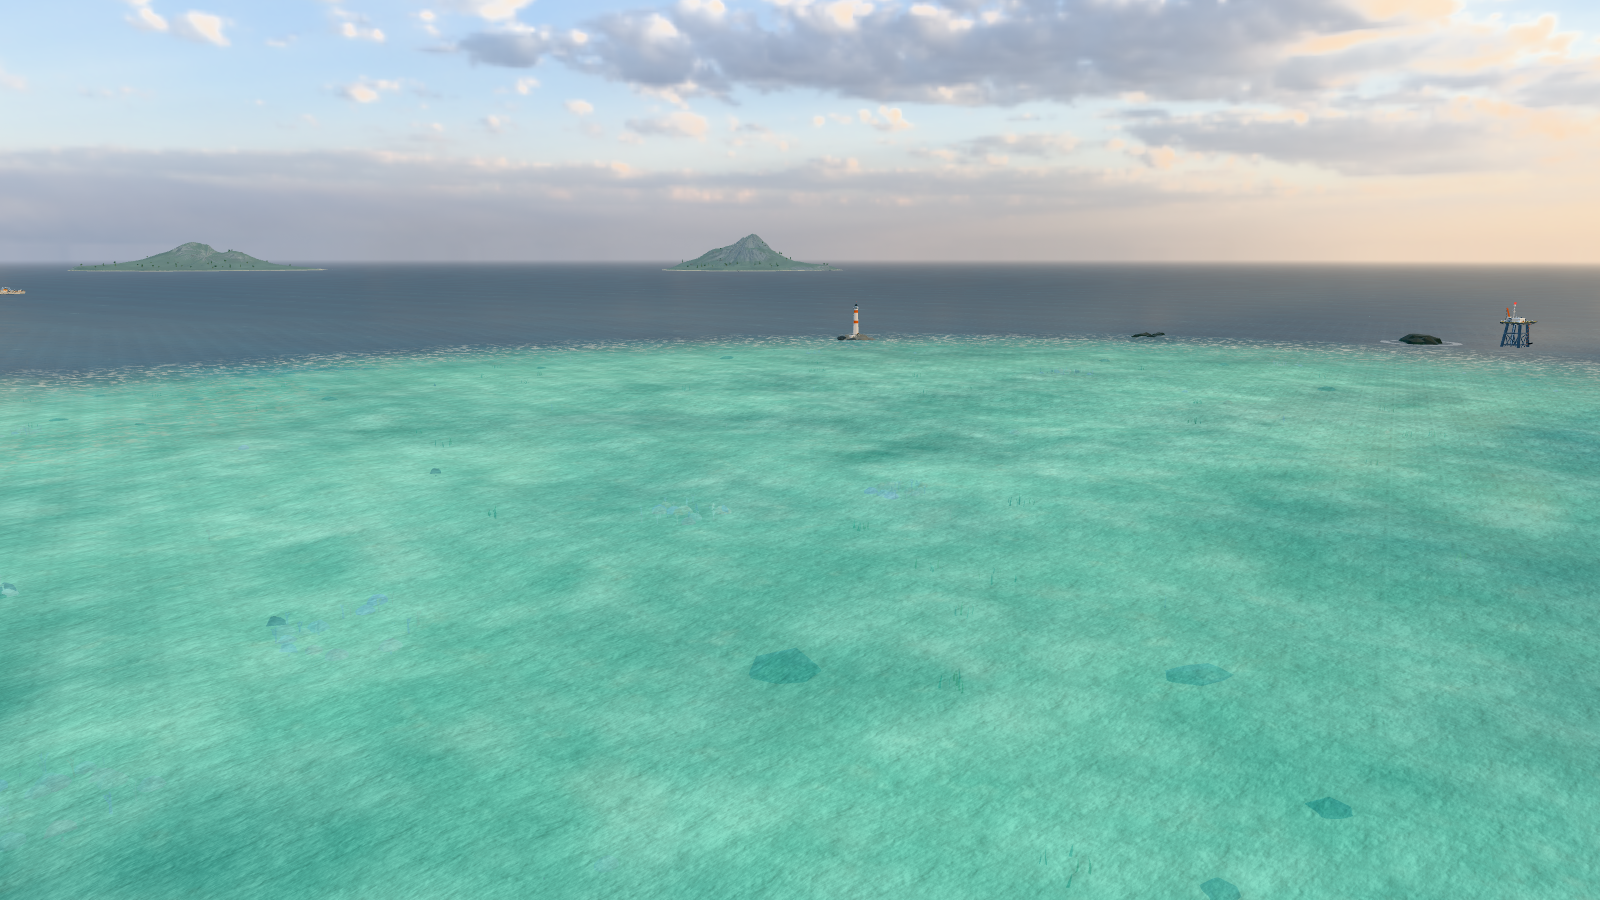
\includegraphics[width=0.95\linewidth]{figures/fig-04-reef.png}
  \caption{浅海珊瑚礁潟湖：海面半透明，海底沙脊、暗色礁斑、珊瑚与海草透水可见。}
  \label{fig:reef}
\end{figure}

% -----------------------------------------------------------------------------
\section{天空、大气与光照}

v1.0 的天空由程序化渐变穹顶、画布云精灵、卷云平面与太阳光晕构成；v1.1 把整个大气替换为一张本地存放的 Poly Haven 全景 HDR：“Kloppenheim 06 (Pure Sky)”，2K 等距圆柱投影（$2048\times1024$，Radiance RGBE），CC0 1.0 许可。改用实拍全景而非继续程序化的原因有三：其一，真实的云与太阳具有程序化噪声难以复现的方向性结构（逆光积云的金边、被云遮挡的柔和太阳）；其二，海面菲涅尔反射与远处雾色可以直接采样同一张图，天与海在任何视角下都同源；其三，金属与玻璃的图像环境光（IBL）与可见天空一致，不再需要另一套程序化立方图。

\subsection{HDR 天空穹顶}

天空仍由一个跟随相机的巨大穹顶（半径 48\,km）与专用 ShaderMaterial 绘制，但片元着色器不再合成天空，而是对 HDR 全景作等距圆柱投影采样：

\begin{itemize}
  \item \textbf{等距圆柱映射}：three.js 的 equirectangular 约定为 $u=\operatorname{atan2}(z,x)/2\pi+0.5$、$v=\arcsin y/\pi+0.5$；\texttt{EquirectangularReflectionMapping} 与全景文件的朝向（\texttt{flipY} 保持默认 \texttt{true}）一致，方位角 $0^\circ$ 指向 $+X$、$90^\circ$ 指向 $+Z$，行 0 为天顶；
  \item \textbf{采样约定}：全景按固定方位采样（不做额外偏航）；\texttt{wrapS = RepeatWrapping} 消除 $u=0/1$ 处 atan2 接缝在 mip 采样下形成的模糊竖带，\texttt{wrapT} 保持 clamp；开启 mipmap 与各向异性过滤（上限 8），保证环绕视角下地平线不闪烁；
  \item \textbf{地平线以下}：采样前把视线方向钳制在 \texttt{d.y = max(d.y, 0.006)}，穹顶因此不会把全景中“镜像的下半球”当作天空；穹顶在地平线以下用同一钳制采样到的地平线颜色向更深、更雾的方向延展，使远处海面网格的边缘也融进同一片天空（海面反射使用更粗的 mip，模糊核会在地平线附近掠过少量下半球像素，但那里是上半球的连续模糊镜像，不会出现双重云）；
  \item \textbf{色调与抖动}：全景辐射值乘以 \texttt{hdrIntensity}（0.9）后交给 \texttt{NeutralToneMapping}（曝光 1.0）输出；坐标哈希抖动消除平滑天空的 8-bit 色带；
  \item \textbf{回退}：若本地 HDR 缺失或解码失败，着色器切换到原有程序化路径（\texttt{skyTint()} 渐变 + 太阳圆盘与光晕），场景不中断。
\end{itemize}

穹顶材质关闭深度测试与深度写入，并设置 \texttt{renderOrder = -1000}，保证它永远在所有不透明物体之后、其他半透明物体之前绘制。

\subsection{海天无缝：同一张 HDR 的地平线与反射}

海面与天空现在共享的不再是一段解析颜色函数，而是同一张 HDR 全景：

\begin{itemize}
  \item \textbf{反射}：以水平面镜面方向与波浪法线方向分别从全景的模糊 mip（约 4.6 / 5.6 级）采样并混合，乘以菲涅尔系数——HDR 地平线比旧的程序化天空亮得多，因此反射项整体缩放到 0.48、菲涅尔上限压到 0.40，近中景仍保持青蓝色水体色，而碎浪与远处海面获得真实的暖/冷反射层次；
  \item \textbf{逐方向雾}：远处海面的指数雾目标色取该视线水平方向的 HDR 地平线颜色（\texttt{skyRadiance()}），因此太阳一侧的地平线自动偏暖金、背光侧偏冷蓝，天与海在像素级连续，不需要“地平线雾墙”或背景板；
  \item \textbf{太阳对齐}：主光、补光与着色器中的太阳方向都与全景中烘焙的太阳（方位角 $40.69^\circ$、仰角 $4.66^\circ$）一致，海面碎金反射带、云的金边与船体的受光面因此指向同一个太阳（图~\ref{fig:side}）。
\end{itemize}

\begin{figure}[H]
  \centering
  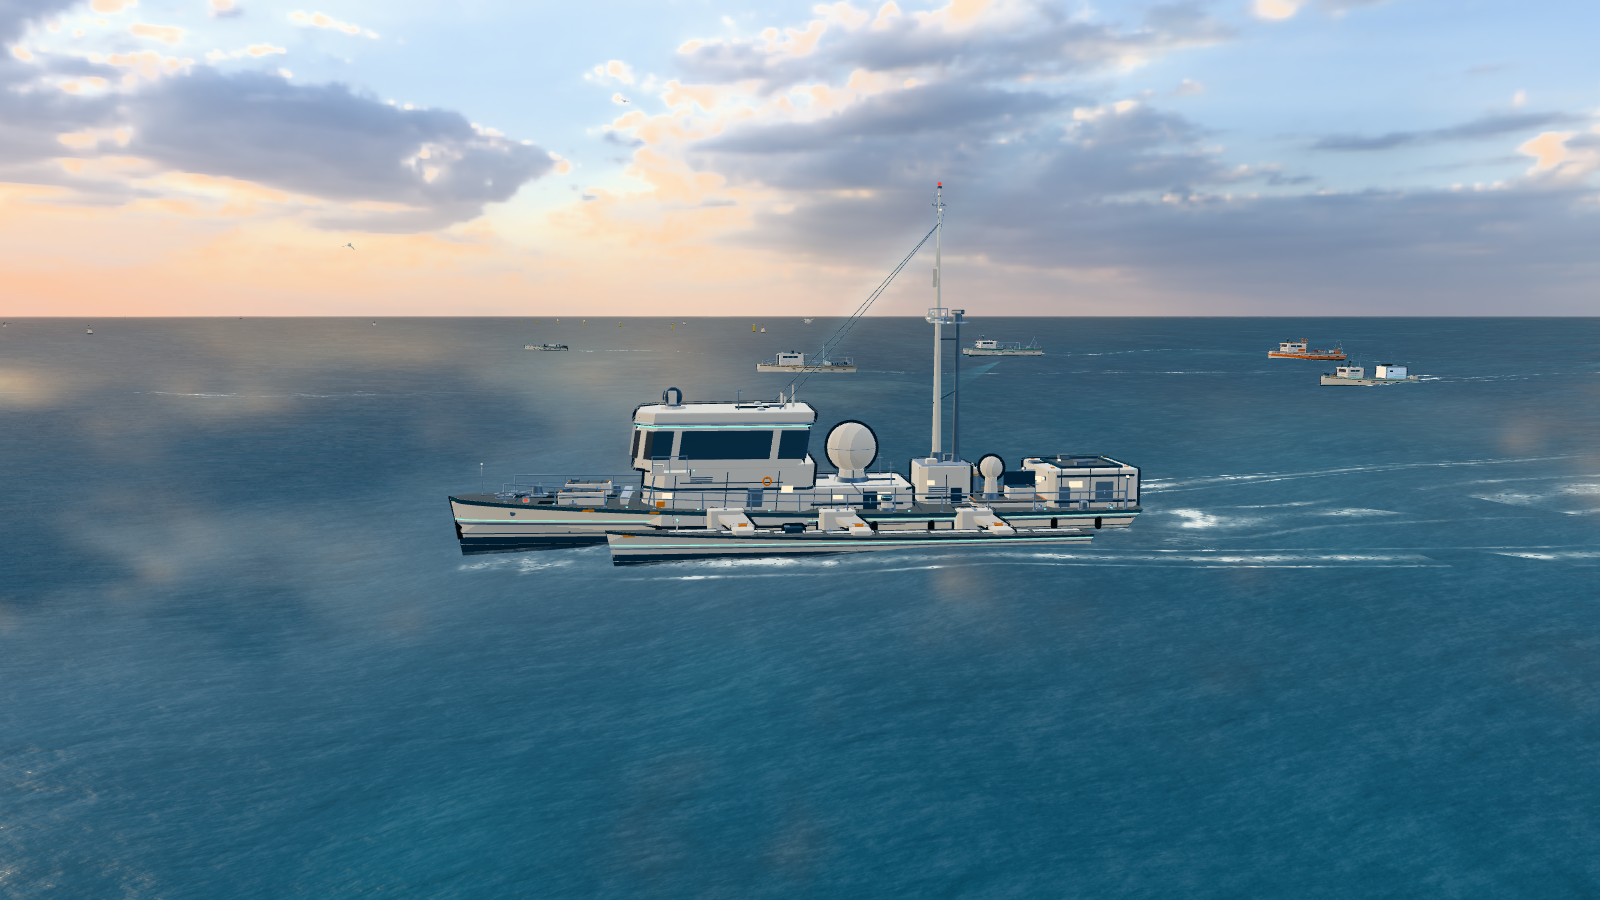
\includegraphics[width=0.95\linewidth]{figures/fig-07-side.png}
  \caption{低角度侧视：HDR 天空的逆光积云、海天交界线与船体边缘光。}
  \label{fig:side}
\end{figure}

\subsection{云与太阳：来自全景的内容}

v1.0 的三层程序化云（26 个积云精灵、5 张卷云平面、1 个太阳光晕精灵）已全部移除；云与太阳现在完全来自 HDR 全景本身，因此环绕相机时会看到真实的全景内容：

\begin{itemize}
  \item \textbf{太阳扇区（方位 $0^\circ$--$90^\circ$）}：金色低角度太阳藏在薄云之后，暖色霞光、逆光积云的亮边与放射状光束；
  \item \textbf{其他方位}：散布的积云带与云影，方位 $120^\circ$--$300^\circ$ 为对比度很低的深蓝天顶；全景在水平方向无缝（wrap 列差异 $<1\%$）；
  \item \textbf{不再有精灵}：没有公告板云、没有水平卷云平面、没有加法混合的太阳光晕，也没有随时间漂移的云层动画——天空是静态的真实大气，场景中的动态全部来自海面、尾迹与舰艇。
\end{itemize}

\subsection{加载、许可与替换}

HDR 全景由 \file{src/core/hdri.js} 加载：\texttt{HDRLoader} 读入 RGBE 纹理（\texttt{LinearSRGBColorSpace}，\texttt{flipY} 保持 true），再由 \texttt{PMREMGenerator} 预滤波为环境图供金属/玻璃使用；同一张纹理以 uniform 形式同时供天空穹顶与海面着色器采样。文件随仓库分发，从应用自身 base URL 同源加载，运行时不访问网络：

\begin{center}\small
\file{public/hdr/kloppenheim\_06\_puresky\_2k.hdr}\\[0.25em]
4\,434\,394 字节（Radiance RGBE，$2048\times1024$），MD5 \texttt{590a829b3cf71216451655e601d542c6}
\end{center}

素材信息：Poly Haven “Kloppenheim 06 (Pure Sky)”——Greg Zaal（原始全景）、Jarod Guest（天空编辑），CC0 1.0 Universal 公有领域贡献，\url{https://polyhaven.com/a/kloppenheim_06_puresky}；完整署名与替换方法见仓库根目录 \file{CREDITS.md}。替换全景时保持 2:1 等距圆柱投影，更新 \file{config.js} 中 \texttt{WORLD.sky.hdrPath}；若太阳位置不同，同步更新 \texttt{WORLD.sunDirection}（主光、补光、天空与海面的 \texttt{uSunDir} uniform 都由它派生）以及 \texttt{sunColor} / \texttt{sunIntensity}。

另一项本地素材是水面法线贴图（three.js 官方示例纹理，MIT 许可），其加载与三层复用见 §4.4，许可与替换方法同样记录在 \file{CREDITS.md}。

\subsection{光照与材质响应}

场景采用“暖色低角度主光 + 冷色半球环境光 + 冷色补光 + HDR 环境反射”的方案（表~\ref{tab:lights}）。主光的方向、颜色与强度按全景中烘焙的太阳重新标定：方位角 $40.7^\circ$、仰角 $4.7^\circ$，色温偏暖（\texttt{0xffd9a6}）。实时阴影仍然关闭：一方面海面使用自定义 ShaderMaterial，接入阴影贴图的成本与复杂度较高；另一方面三渲二风格通过卡通阶跃光照、边缘光与假接触泡沫已经足以表达体积。船体与水面之间通过尾迹泡沫、船首破浪与水线压暗来建立接触关系。

\begin{table}[H]
\centering
\caption{光照配置（v1.1，HDR 天空）}
\label{tab:lights}
\small
\begin{tabular}{@{}p{0.21\linewidth}p{0.34\linewidth}p{0.13\linewidth}p{0.26\linewidth}@{}}
\toprule
\textbf{光源} & \textbf{颜色} & \textbf{强度} & \textbf{方向/作用} \\
\midrule
平行光（太阳） & \texttt{0xffd9a6} 暖白 & 1.85 & 方位角 $40.7^\circ$、仰角 $4.7^\circ$，与 HDR 太阳对齐 \\
半球光 & 天 \texttt{0xc7dcf0} / 地 \texttt{0x2a5a6c} & 1.18 & 填充背光面，形成蓝灰阴影 \\
平行光（补光） & \texttt{0xbcd6ee} 冷蓝 & 0.50 & 从太阳反方向补冷光，增强轮廓 \\
HDR 环境反射 & “Kloppenheim 06” PMREM & 0.9$^{\dagger}$ & 金属、玻璃的环境光与反射（IBL） \\
\bottomrule
\end{tabular}
\vspace{0.3em}
{\footnotesize $^{\dagger}$ \texttt{WORLD.sky.hdrIntensity}，同时作用于天空穹顶与海面采样；环境图取自同一全景。}
\end{table}

% -----------------------------------------------------------------------------
\section{无人艇程序化建模}

\subsection{统一设计语言与尺度}

全部 17 艘无人艇遵循统一工业设计语言：修长船体、低矮封闭设备舱、模块化任务载荷、深色玻璃传感器窗口、珍珠白 + 海军灰 + 深海军蓝涂装，少量信号橙与荧光青作为识别色。尺寸覆盖 10.5--30~m，旗舰作为尺度参照（表~\ref{tab:boats}）。

\begin{table}[H]
\centering
\caption{无人艇类别与主要参数}
\label{tab:boats}
\small
\begin{tabular}{@{}lccccp{0.40\linewidth}@{}}
\toprule
\textbf{类别} & \textbf{数量} & \textbf{长度}/m & \textbf{型宽}/m & \textbf{吃水}/m & \textbf{主要特征} \\
\midrule
旗舰 & 1 & 30.0 & 9.4 & 1.7 & 三体、双雷达罩、通信桅杆、旋转雷达、光电球、UUV 机库、折臂吊 \\
侦察艇 & 5 & 10.5 & 3.0 & 0.62 & 深 V 高速艇体、喷水推进、球形光电、扫描雷达、橙/青识别区 \\
环境监测 & 3 & 16.5 & 5.6 & 1.0 & 实验室舱、尾部自动采样平台、升降机构、采样瓶架、折叠探针 \\
海洋测绘 & 2 & 18.0 & 7.4 & 1.1 & 对称双体、中央传感器通道、声呐吊舱、A 形门架、双 GNSS 罩 \\
多用途巡逻 & 2 & 14.5 & 4.7 & 0.9 & 模块化任务集装箱、雷达、光电、双天线 \\
通信中继 & 1 & 19.0 & 6.2 & 1.15 & 11~m 桁架桅杆、多组微波天线、卫星罩、索槽 \\
能源保障 & 2 & 20.0 & 7.0 & 1.2 & 电池柜阵列、太阳能板、甲板吊、充电卷盘、维护平台 \\
无人救援 & 1 & 15.5 & 5.4 & 1.0 & 橙白涂装、救援平台、折臂、救生圈发射架、担架 \\
\bottomrule
\end{tabular}
\end{table}

\subsection{参数化船体生成}

每条船体由 \file{core/geo.js} 中的 \texttt{hullParts(spec)} 生成。其核心是把船体看作沿长度方向变化的横截面族：对参数 $u\in[0,1]$（船尾到船首）定义半宽、吃水、干舷、外飘、艏柱前倾与截面幂次，再用密排截面放样成网格（代码~\ref{lst:hull}）。

\begin{lstlisting}[language=Java, caption={参数化船体截面与船体部件拆分}, label={lst:hull}]
// spec: length, beam, freeboard, sheer, draft, bowSharp, flare,
//       rocker, sternWidth, camber, sectionPower, rake
const parts = hullParts({
  length: 30, beam: 5.6, freeboard: 1.46, sheer: 0.74,
  draft: 1.635, bowSharp: 1.16, flare: 0.3, rocker: 0.55,
  sectionPower: 1.72, rake: 0.24, uSegments: 56,
});
// parts = { lower, topsides, deck, transom }
// lower    -> keel to waterline (deep navy antifouling)
// topsides -> waterline to gunwale (pearl white)
// deck     -> cambered deck cap
// transom  -> flat stern panel
\end{lstlisting}

上下两部分独立生成、共享水线顶点，因此水线是一条干净锐利的色阶分界，而不是插值渐变；再叠加 \texttt{hullBand()} 生成的深蓝腰线、金属护舷条与青色识别灯带。该方法同时服务于单体艇、双体测绘艇的两片船体与三体旗舰的中央主船体/两个浮体。

\subsection{Builder：合批、描边与动态部件}

逐零件建模会产生成千上万个 Mesh。\file{core/geo.js} 的 \texttt{Builder} 负责将静态几何按材质键合并为不超过 10 余个网格，并额外生成一个“反向外壳”描边网格（代码~\ref{lst:builder}）。

\begin{lstlisting}[language=Java, caption={Builder 的典型用法}, label={lst:builder}]
const b = new Builder(materials, { outlineMaterial: materials.outlineBoat });
b.solid(parts.lower,  'hullBottom', { pos });   // merged + outline
b.solid(parts.topsides,'pearl',    { pos });
b.add(railing,        'metal',     { pos: [...] });  // merge only
const radar = b.dynamic('radar');               // animated sub-group
radar.add(new THREE.Mesh(radarBarGeo, materials.metalDark));
const group = b.build();                        // 1 draw per material + outline
\end{lstlisting}

描边材质为背面材质，顶点着色器中沿法线向外扩张固定宽度（约 0.13~m），形成干净的三渲二轮廓线，同时不产生额外的屏幕空间后处理开销。

\subsection{旗舰设计}

旗舰是本场景的核心视觉焦点，采用三体结构：中央主船体长 30~m，两侧各一个 20~m 浮体（间距 3.94~m），通过三组后掠横臂与斜撑连接；船体为尖锐破浪艏、低重心、宽阔中央任务甲板与流线型外壳。主要构成：

\begin{itemize}
  \item \textbf{上层建筑}：前部后掠式驾驶/设备舱，环绕式深色玻璃带，珍珠白折面舱顶，青色灯带与暖色工作窗；
  \item \textbf{感知设备}：大型白色卫通雷达罩（半径 1.1~m）、后部小型雷达罩、8~m 通信桅杆、多组刀形天线、旋转式海事雷达、前部可转光电球、圆柱激光雷达、气象站；
  \item \textbf{任务设备}：后部 UUV 机库（带凹陷式艉门与橙色警示条纹）、折叠关节吊臂、模块化任务舱口、甲板系缆桩与检修舱盖；
  \item \textbf{细节}：黑色橡胶分段护舷、嵌入式金属护栏、排水孔、冷却格栅、面板接缝、航行灯（左红右绿）、桅顶白灯、青色识别灯带；
  \item \textbf{动态部件}：旋转雷达、缓慢扫描的光电云台、周期闪烁的桅顶警示灯。
\end{itemize}

旗舰共 61\,302 个三角形（其中描边约 12.6k），13 个静态材质批次 + 1 个描边 + 3 组动态网格。

\begin{figure}[H]
  \centering
  \begin{subfigure}[b]{0.49\linewidth}
    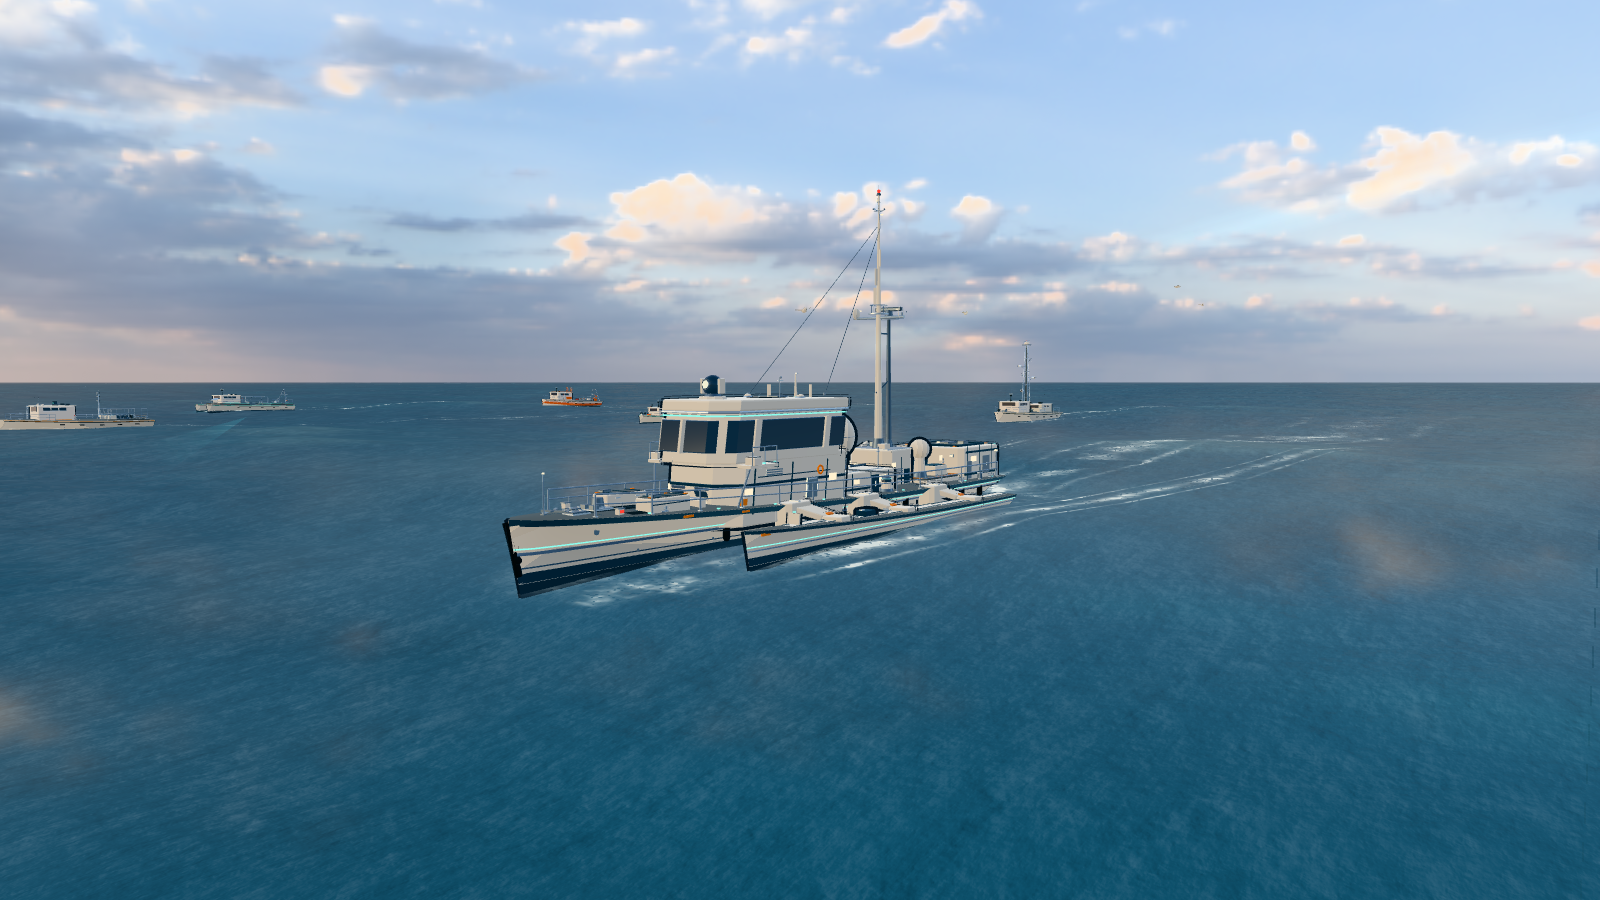
\includegraphics[width=\linewidth]{figures/fig-06-bow.png}
    \caption{旗舰船艏方向}
  \end{subfigure}\hfill
  \begin{subfigure}[b]{0.49\linewidth}
    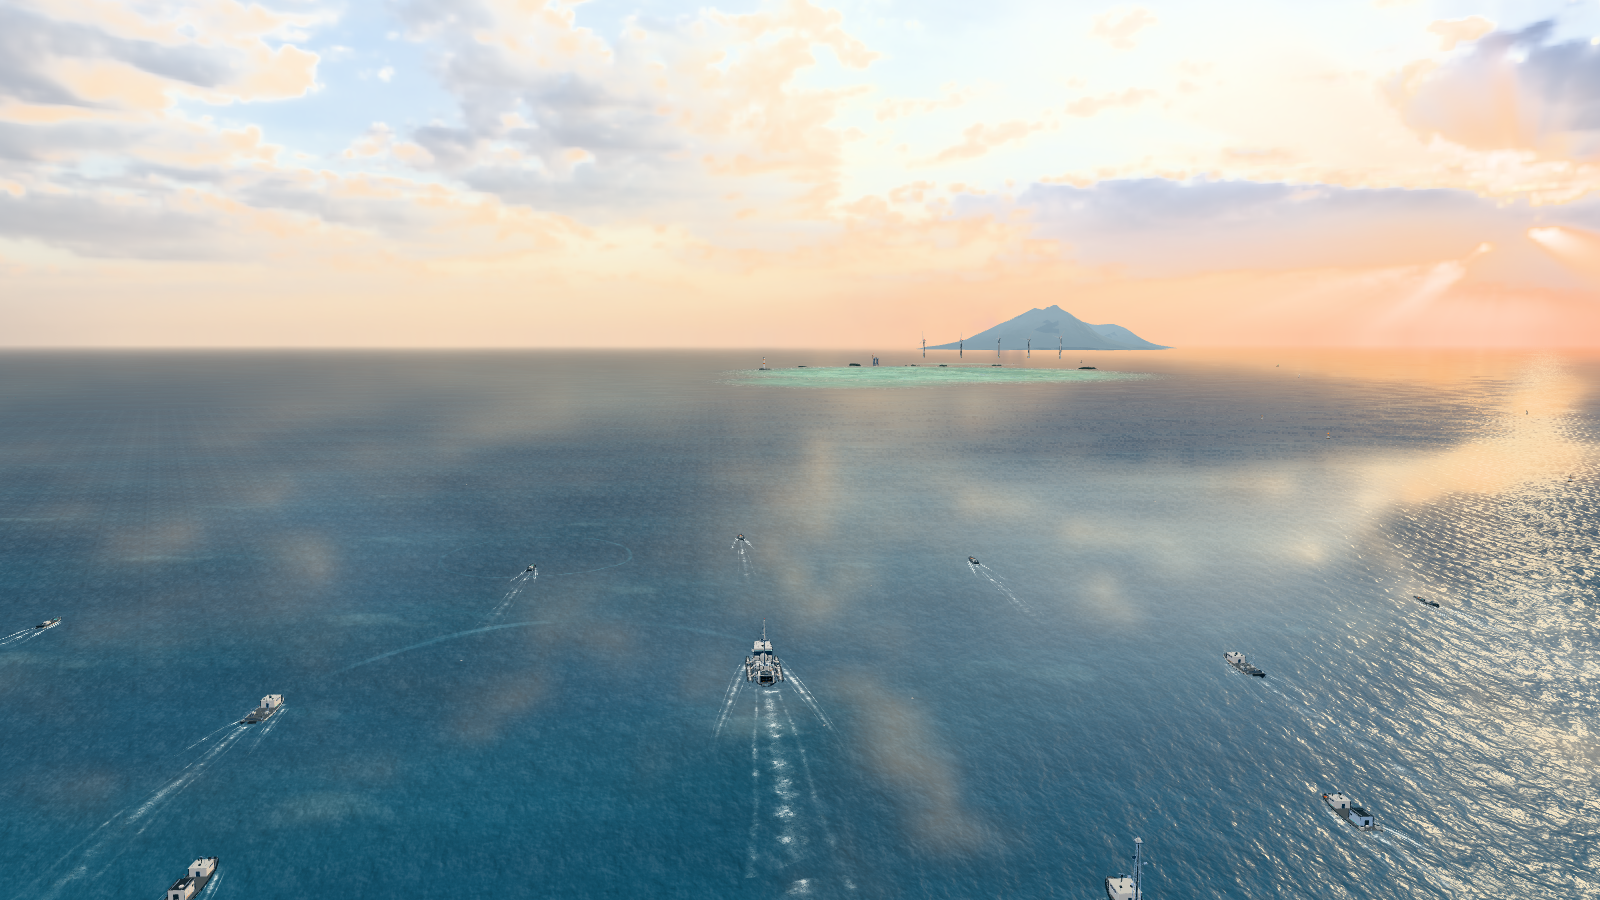
\includegraphics[width=\linewidth]{figures/fig-08-user-swarm.png}
    \caption{编队上空近景}
  \end{subfigure}
  \caption{旗舰与集群实机截图。}
  \label{fig:flagship}
\end{figure}

\subsection{材质库与三渲二外观}

\file{core/materials.js} 集中定义材质：

\begin{itemize}
  \item \textbf{卡通材质}：\texttt{MeshToonMaterial} + 4 阶梯度贴图，并在 \texttt{onBeforeCompile} 中注入菲涅尔边缘光（rim），使背光面仍保持清晰轮廓；
  \item \textbf{金属/玻璃}：\texttt{MeshStandardMaterial} + HDR 全景 PMREM 环境反射（无 HDR 时回退程序化天空立方图），分别控制金属度与粗糙度；
  \item \textbf{发光件}：航行灯、识别灯带、桅灯使用无光照的 Basic 材质；
  \item \textbf{描边}：背面材质 + 顶点法线外扩。
\end{itemize}

% -----------------------------------------------------------------------------
\section{编队动力学与航行}

\subsection{航线}

编队沿一条极宽的左转圆弧前进。设航向角 $\theta(t)$ 随时间线性增加，则旗舰轨迹可由积分得到解析式：

\begin{equation}
\begin{aligned}
x(t) &= x_0 + \frac{v}{\omega}\big(\sin\theta(t)-\sin\theta_0\big),\\
z(t) &= z_0 + \frac{v}{\omega}\big(\cos\theta(t)-\cos\theta_0\big),
\end{aligned}
\qquad \theta(t)=\theta_0+\omega t,
\end{equation}

其中 $v=3.1$~m/s，$\omega=0.0019$~rad/s，转弯半径约 1.63~km。该半径使编队在数分钟内只缓慢改变航向，形成“宽阔弧形转弯”的视觉效果，同时不会让相机跟随产生突兀旋转。

\subsection{阵位与自然摆动}

17 艘舰艇在“编队坐标系”（前向 $+$、右向 $+$）中拥有固定阵位：旗舰位于原点；5 艘侦察艇在正前方 46--186~m 呈箭头展开；两侧中型艇在 $-268$~m 至 $+224$~m 的横向范围内错列；4 艘保障艇位于后方 118--134~m。阵位之上叠加多组低频正弦摆动，使编队保持严谨秩序的同时具有自然呼吸感；侦察艇还额外叠加周期性横向展开项，模拟“向外搜索—回归编队”的行为。

\subsection{跟随与航向控制}

每艘艇用指数弹簧逼近目标阵位（式~\ref{eq:spring}），并用“航路方向 + 位置修正”的混合向量计算期望航向，再对航向做角度平滑，从而在转弯时自然出现内切与外扩：

\begin{equation}
\mathbf{p}_{k+1}=\mathbf{p}_k+\big(\mathbf{p}^{\ast}-\mathbf{p}_k\big)\left(1-e^{-dt/\tau}\right),
\qquad
\psi^{\ast}=\arg\Big(\mathbf{d}_{course}+\alpha(\mathbf{p}^{\ast}-\mathbf{p})\Big).
\label{eq:spring}
\end{equation}

不同吨位的跟随时间常数 $\tau$ 与转向响应不同，使小艇更灵活、保障艇更沉稳。转弯时根据角速度给高速艇叠加轻微侧倾（bank）。

\subsection{随浪姿态}

船体姿态不使用解析波梯度直接计算，而是对船体“首、尾、左、右”四个点采样水面高度，再按船长与型宽求纵摇与横摇（式~\ref{eq:attitude}）。这样 30~m 的旗舰不会被 5~m 的细浪直接抬起，姿态被船体尺度自然低通，同时小船仍然灵活。

\begin{equation}
\begin{aligned}
\text{pitch}^{\ast} &= \arctan\frac{h_{bow}-h_{stern}}{2L_h}\,\gamma_p + \text{planing},\\
\text{roll}^{\ast} &= -\arctan\frac{h_{right}-h_{left}}{2B_h}\,\gamma_r + \text{bank},\\
h_{heave}^{\ast} &= 0.35\,h_c + 0.1625\,(h_b+h_s+h_r+h_l),
\end{aligned}
\label{eq:attitude}
\end{equation}

其中 $\gamma_p,\gamma_r$ 为按艇型配置的响应系数（高速艇接近 1，双体测绘艇约 0.4）。升沉、纵摇、横摇均经过指数平滑，避免数值抖动。

\begin{figure}[H]
  \centering
  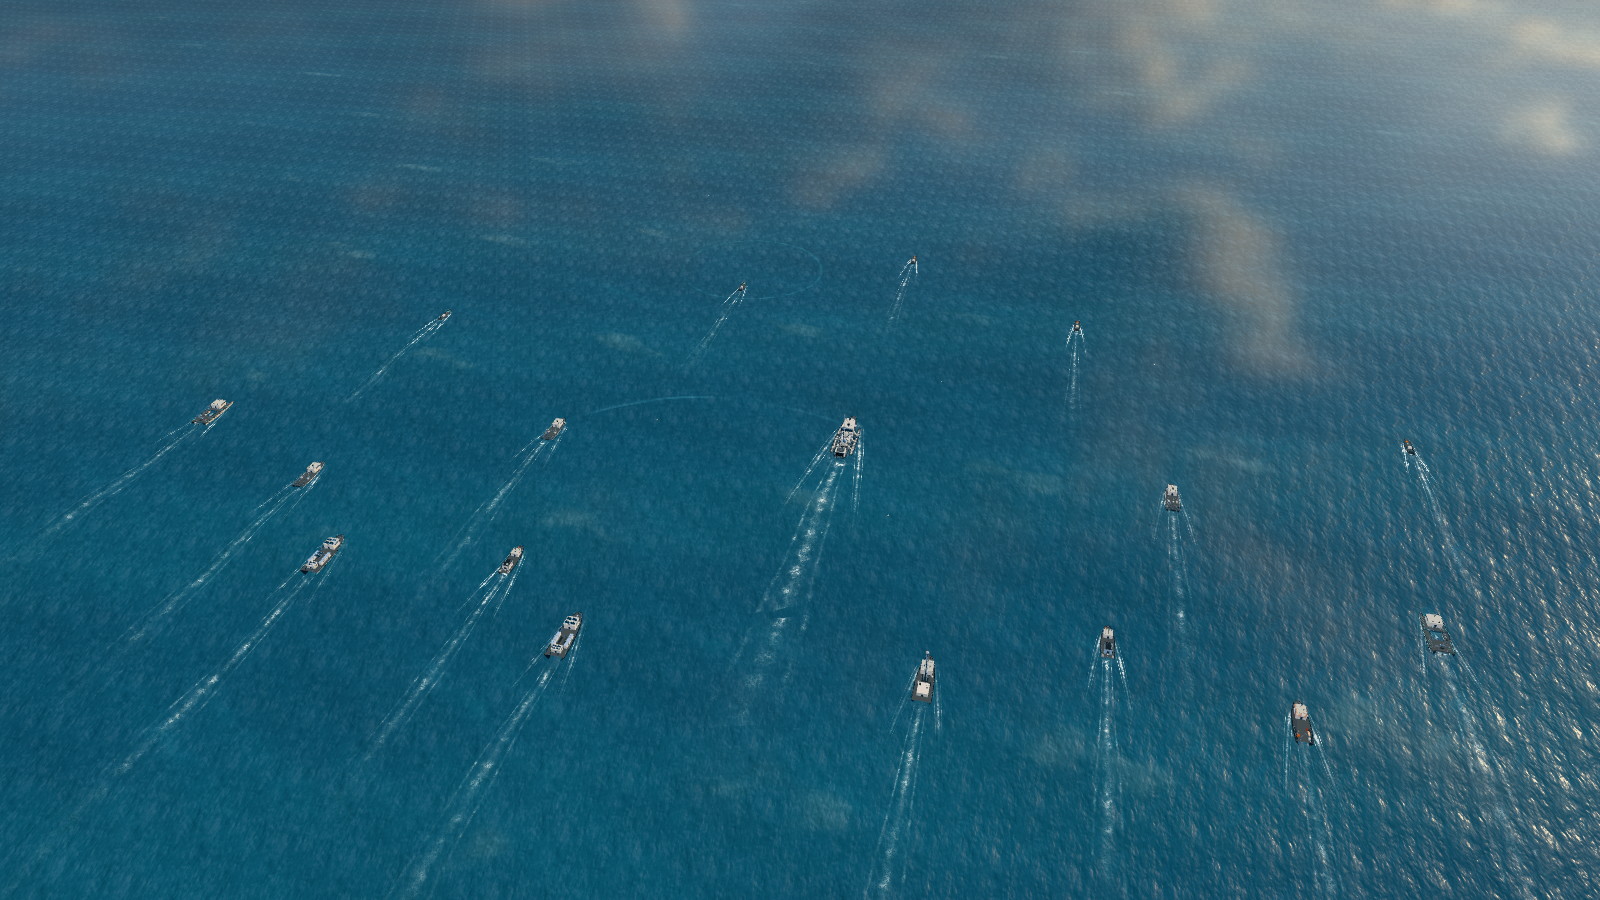
\includegraphics[width=0.95\linewidth]{figures/fig-02-fleet.png}
  \caption{高空俯视：17 艘舰艇的编队秩序、航向与 17 条白色尾迹。}
  \label{fig:fleet}
\end{figure}

% -----------------------------------------------------------------------------
\section{尾迹、泡沫与协同光效}

\subsection{历史轨迹尾迹}

每艘船保存两条世界坐标历史缓冲：近端 32 个采样点（每 0.1~s 一个，约 3.2~s）与稀疏长尾 128 个点（每 0.5~s 一个，最长约 55~s）。每帧根据最近采样点重建一条包含 46 个横截面的尾迹带：

\begin{itemize}
  \item 每个横截面根据船体航向计算左右方向，宽度随“年龄”从约 $0.60\times W_{wake}$ 扩展到 $2.4$--$3.1\times W_{wake}$；
  \item 顶点高度实时采样共享波场，使尾迹贴合起伏的海面而不是悬空平面；
  \item 每条尾迹约 90--160 个三角形，使用动态缓冲原地更新，不产生每帧临时对象。
\end{itemize}

\subsection{泡沫着色器}

尾迹使用统一的自定义 ShaderMaterial，按几何类型分为：中央尾迹带、船首两条 V 形扩散臂、船体两侧水线泡沫线、船首泡沫项圈、尾部推进泡沫与扰动区。片元着色器用三种噪声叠加出世界坐标系的泡沫场：

\begin{itemize}
  \item 泡沫沿航行方向缓慢流动，并随“年龄”衰减透明度；
  \item 中央亮带 + 两条边缘细带形成破浪结构，船首 V 臂额外增亮；
  \item 大尺度斑块与小尺度空洞让泡沫呈“被搅动的含气水”而不是一块白色平面；
  \item 冷色泡沫阴影与暖色受光面混合，最后按距离做大气衰减。
\end{itemize}

\subsection{协同可视化光效}

为表达“集群智能”，场景加入极克制的科技光效（全部不使用文字、数字与面板）：

\begin{itemize}
  \item \textbf{通信弧}：6 条低透明度加法混合弧线，在旗舰与协同艇之间短距离连接，光脉冲沿弧线行进，周期 38--62~s、出现时长 12--18~s、透明度仅 0.05--0.09；
  \item \textbf{扫描环}：侦察艇前方偶尔出现的水面扩散圆环，低透明度、短暂；
  \item \textbf{测绘扇形}：测绘艇下方极淡的水下扇形探测光束，周期脉冲。
\end{itemize}

\subsection{海鸥}

8 只程序化低模海鸥在编队附近 8--40~m 高度盘旋，翅膀按“拍动—滑翔”节奏摆动，身体随转弯轻微侧倾，为静态的工业场景加入生命感。

% -----------------------------------------------------------------------------
\section{海域环境构建}

\subsection{海岛地形}

海岛由噪声位移的径向高度场生成，而非圆锥或球体拉伸：

\begin{itemize}
  \item \textbf{近处研究岛}：半径 300~m、最高 92~m。面向船队一侧抬升为分层岩壁与海蚀崖，岛内为起伏绿色丘陵；基地区域被刻出一块约 10--12~m 高的低平海岸台地，供工程建设使用；
  \item \textbf{植被}：两套低模树（细树干 + 多层树冠）以 InstancedMesh 种植 472 棵，避开基地施工区；
  \item \textbf{海岸}：56 块岸石、48 处岩层/海蚀柱、3 条缓慢脉动的拍岸浪环，构成自然的岸线节奏；
  \item \textbf{两座中景岛}（高 220/170~m）：非对称山脊、裸岩带与海蚀柱，颜色随距离变冷；
  \item \textbf{远景岛}（高 430~m）：低模轮廓剪影，在雾气中呈蓝灰色。
\end{itemize}

\begin{figure}[H]
  \centering
  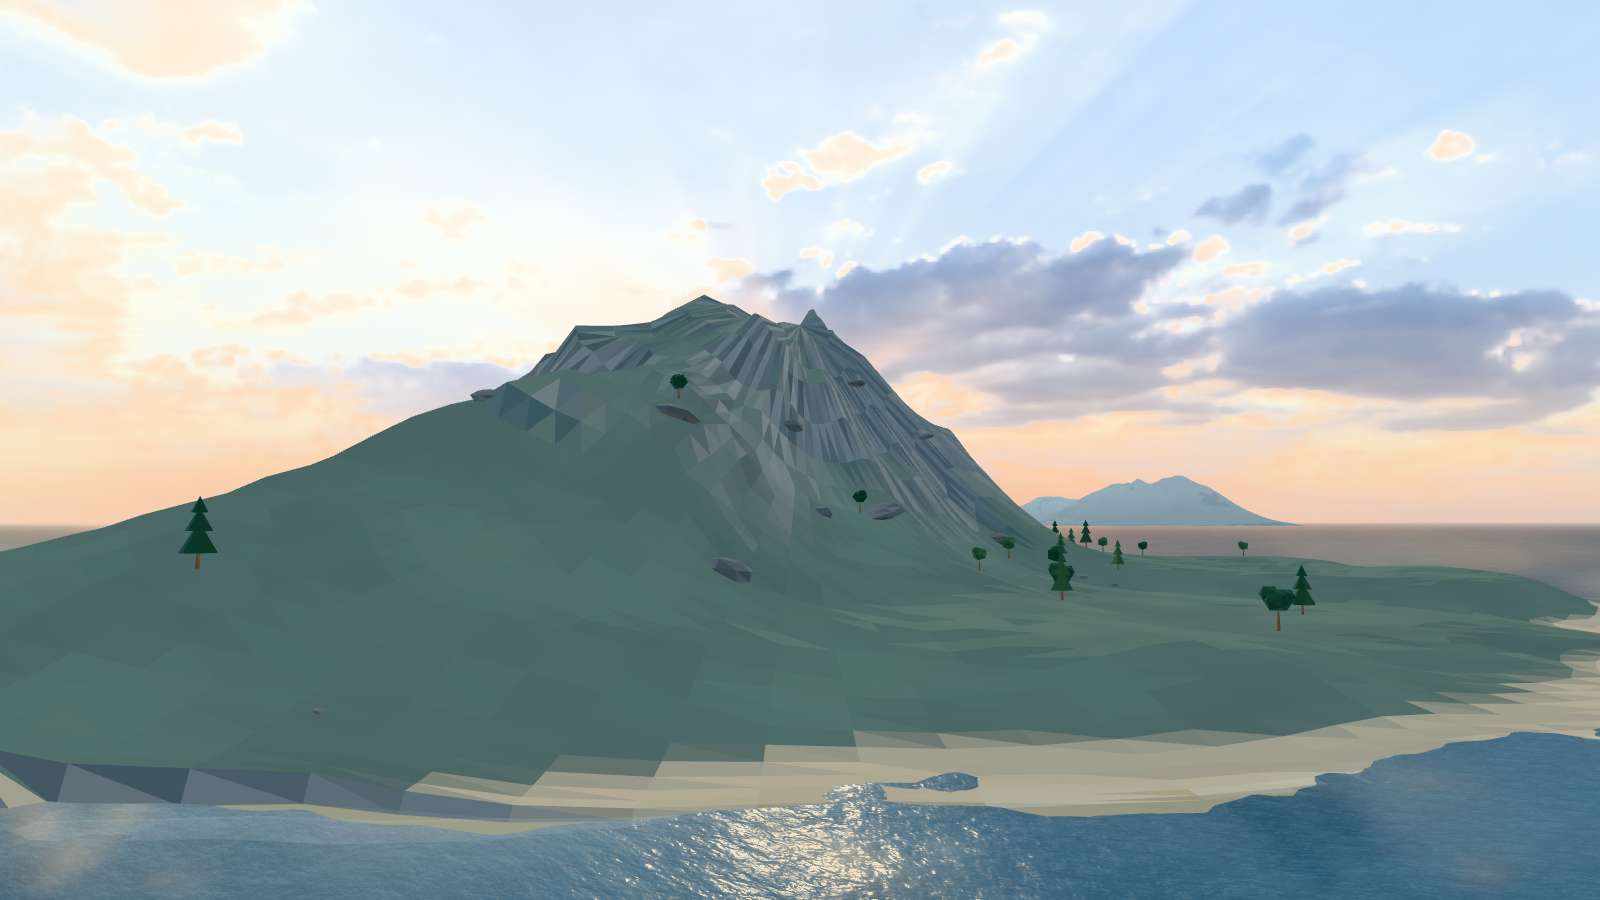
\includegraphics[width=0.95\linewidth]{figures/fig-10-user-island.png}
  \caption{中景海岛近观：低多边形丘陵、裸岩山脊、树木与浅滩沙线。}
  \label{fig:island}
\end{figure}

\subsection{珊瑚礁潟湖}

右侧中景是一片直径约 1.5~km 的浅海珊瑚礁。它由四个椭圆浅滩场驱动，海底为由 224$\times$80 网格构成的平滑沙地（约 4.9 万三角形），叠加：

\begin{itemize}
  \item 498 组珊瑚：分枝状、扇形、脑状/海绵状三类模板，以 InstancedMesh 实例化，色彩为粉、橙、紫三组，簇拥成花园并留出沙质通道；
  \item 661 片随顶点着色器摆动的大型海草；
  \item 52 块水下碎石、7 处露出水面的礁石与两座小礁岛（带泡沫环）；
  \item 3 个鱼群共 136 条小鱼，在珊瑚上方缓慢环绕；
  \item 8 个缓慢漂移的焦散光环。
\end{itemize}

海面在这些浅水区半透明，海底与珊瑚从水面下透出，与无人艇的环境监测/测绘任务形成叙事联系。

\subsection{海上试验基地}

基地位于近岛面向船队一侧，由大型混凝土/岩石平台、防波堤、三组桩基码头与建筑群构成：

\begin{itemize}
  \item \textbf{指挥塔}：约 62~m 高、倾斜切面的塔体，上部深蓝色玻璃观测带、环形外平台、白色雷达罩、旋转雷达与红色航空警示灯；
  \item \textbf{建筑群}：5 栋模块化科研/办公建筑，银白立面、深色玻璃带、屋顶太阳能板与设备；3 条封闭连廊连接；
  \item \textbf{码头}：三组向海伸出的桩基码头（100/125/145~m），防滑甲板、系泊桩、黑色护舷、灯柱、吊机、设备箱与停泊的无人艇；
  \item \textbf{其他}：集装箱堆场、油料/能源模块、太阳能棚、防波堤与灯标。建筑与地形通过地形高度采样函数贴合，不留悬空缝隙。
\end{itemize}

\begin{figure}[H]
  \centering
  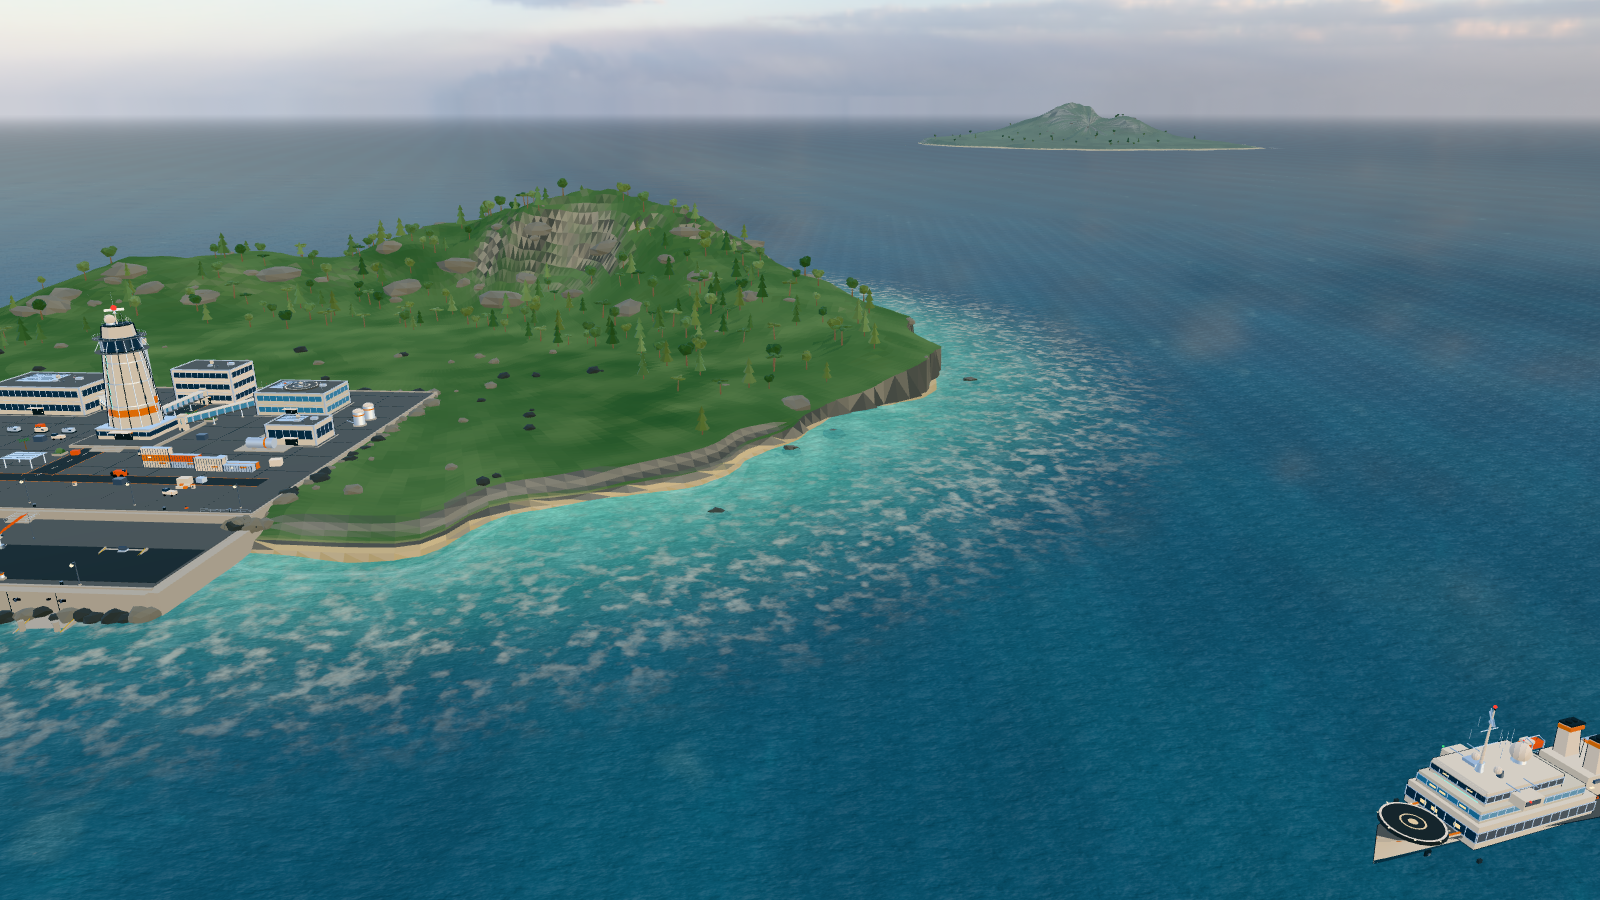
\includegraphics[width=0.95\linewidth]{figures/fig-03-base.png}
  \caption{海上无人系统试验基地：指挥塔、模块建筑、桩基码头、防波堤与停泊艇。}
  \label{fig:base}
\end{figure}

\subsection{母船与航标设施}

\begin{itemize}
  \item \textbf{保障母船}：120~m 级海洋工程船，浅灰白船体、深蓝水线、开放式尾部任务甲板、门式吊机、无人艇停放位、集装箱与通信桅杆，系泊于深水区，缓慢升沉；
  \item \textbf{导航浮标}：18 个智能浮标（橙白涂装、太阳能板、雷达反射器、闪烁信号灯）与黄色航道标、白色科研浮标，全部按共享波场随浪起伏；
  \item \textbf{灯塔}：建在礁石小岛上，约 28~m 白色塔身、观景平台、灯室与暖白旋转灯光；
  \item \textbf{观测平台}：钢制导管架腿 + 甲板 + 设备舱 + 通信桅杆 + 直升机坪的小型自升式平台；
  \item \textbf{海上风电场}：5 台白色风机，塔高约 90--100~m，叶片以不同速率缓慢旋转。
\end{itemize}

\begin{figure}[H]
  \centering
  \begin{subfigure}[b]{0.49\linewidth}
    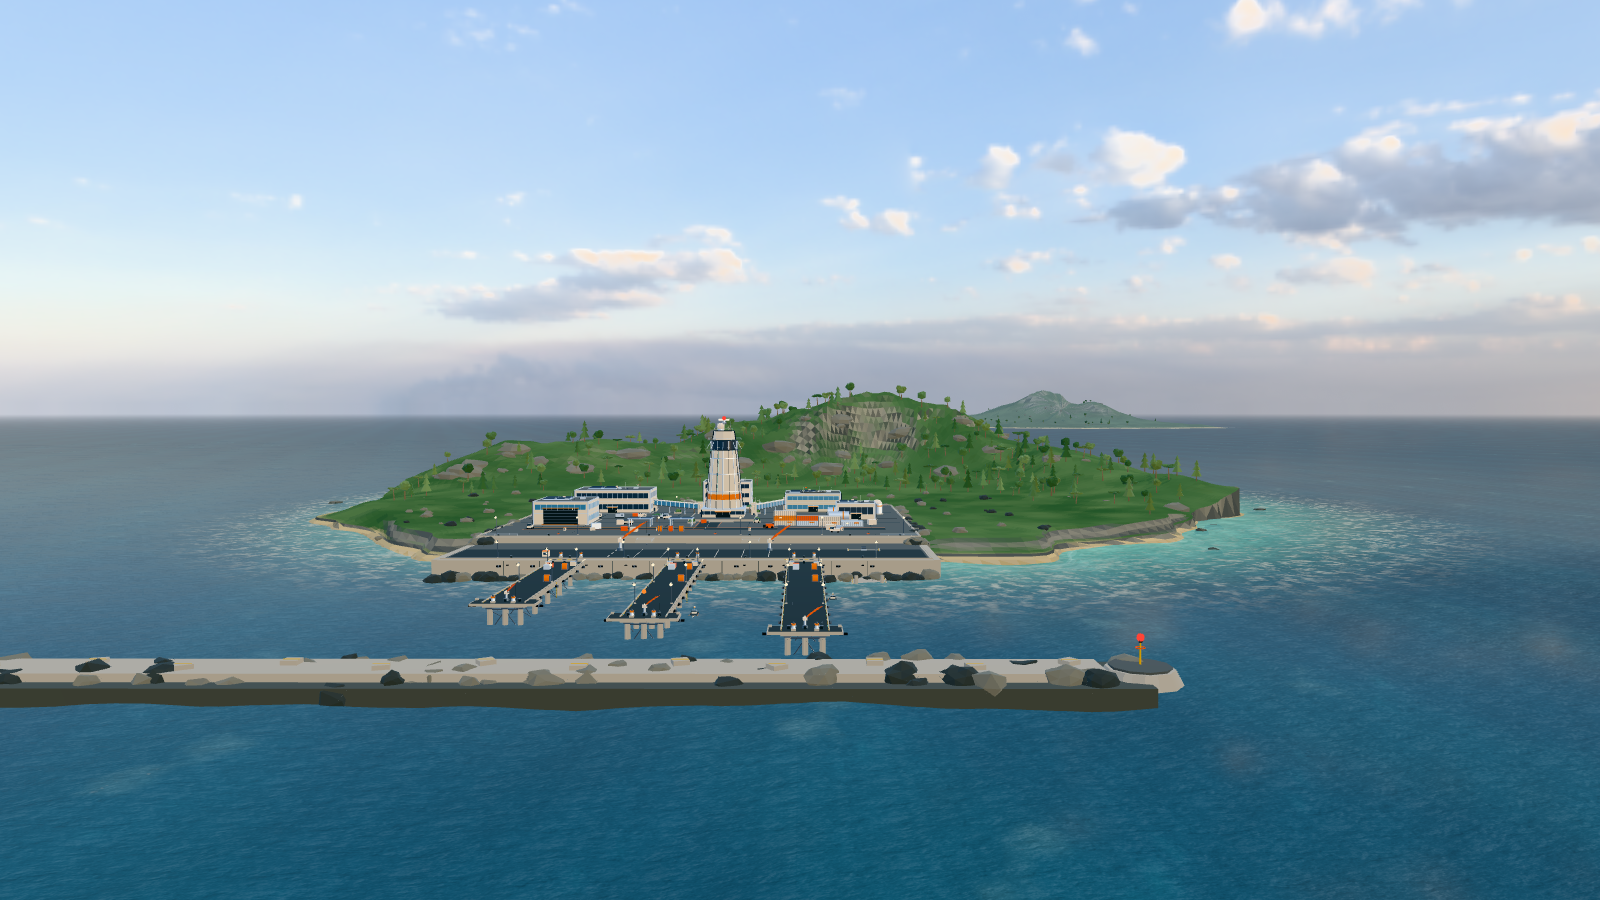
\includegraphics[width=\linewidth]{figures/fig-09-user-base.png}
    \caption{从海面看基地与防波堤}
  \end{subfigure}\hfill
  \begin{subfigure}[b]{0.49\linewidth}
    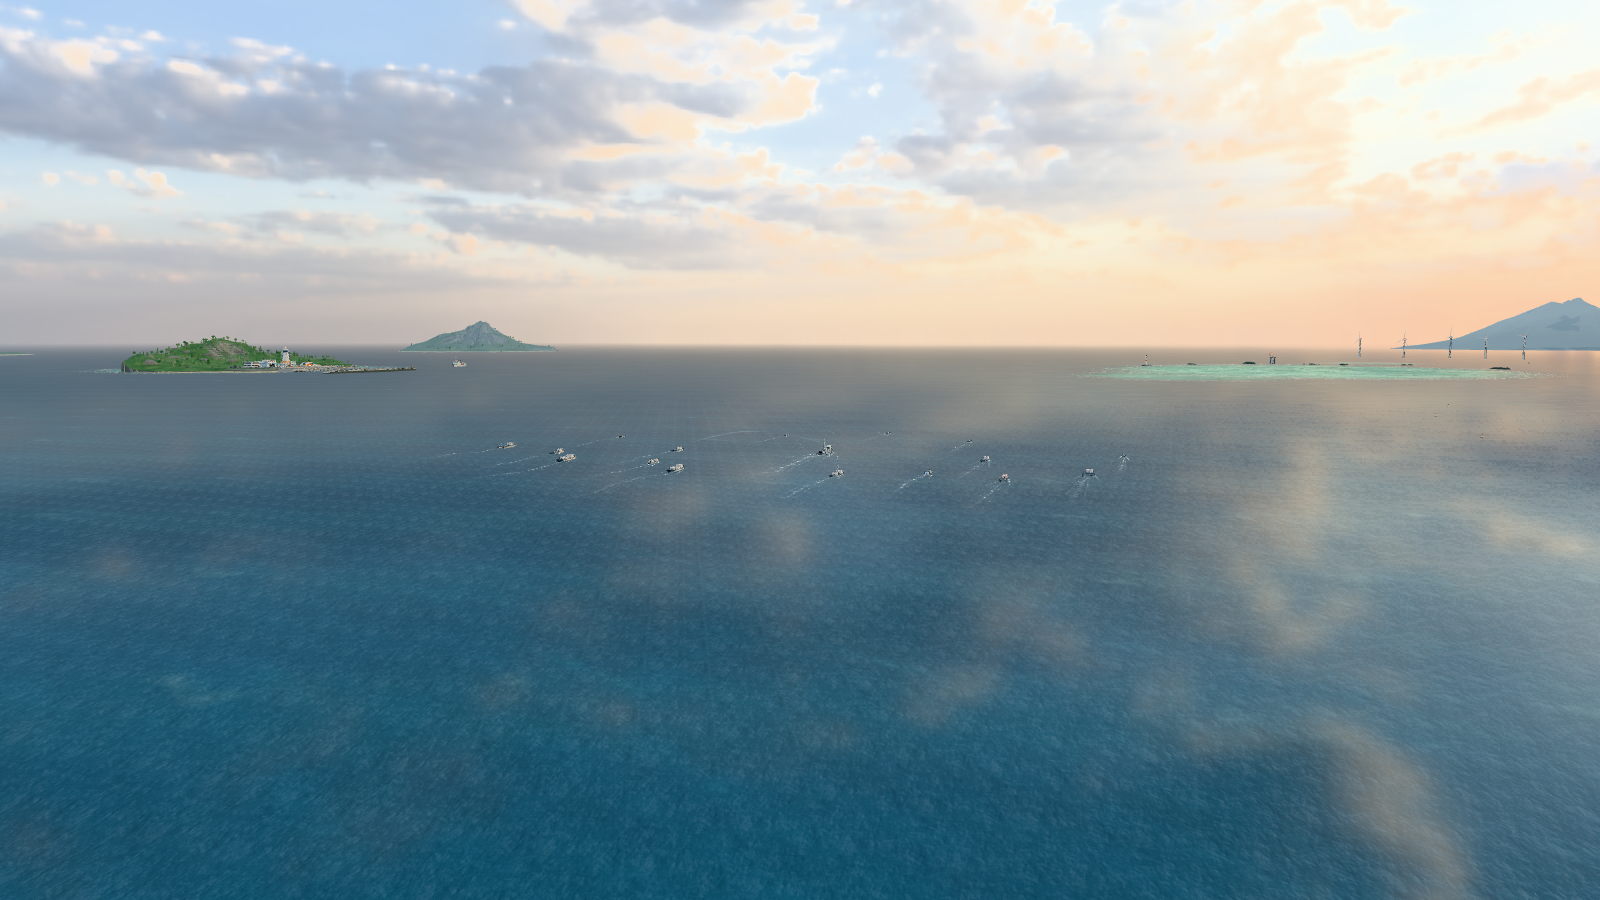
\includegraphics[width=\linewidth]{figures/fig-11-user-wide.png}
    \caption{广角：海岛、基地、编队与海天}
  \end{subfigure}
  \caption{环境实机截图。}
  \label{fig:env-gallery}
\end{figure}

% -----------------------------------------------------------------------------
\section{美术方向、色彩与构图}

\subsection{三渲二的混合管线}

场景并非全部使用卡通材质，而是按物体类型混合多种表现：

\begin{table}[H]
\centering
\caption{不同对象的表现方案}
\label{tab:art}
\small
\begin{tabular}{@{}p{0.20\linewidth}p{0.30\linewidth}p{0.40\linewidth}@{}}
\toprule
\textbf{对象} & \textbf{渲染方式} & \textbf{目的} \\
\midrule
船体/建筑/地形 & 卡通材质 + 4 阶梯度 + 边缘光 & 干净的色块、清晰的轮廓与体积 \\
金属/玻璃 & Standard + HDR PMREM 天空反射 & 工业精密感与真实反射 \\
海面/天空 & 自定义 ShaderMaterial + HDR 全景 + 照片法线 & 程序化波浪、三层法线细节、微明暗、菲涅尔、碎金、HDR 反射、无缝地平线 \\
尾迹/光效 & 半透明自定义着色器 & 泡沫流动、通信光脉冲 \\
描边 & 反向外壳 & 三渲二轮廓，无后处理依赖 \\
\bottomrule
\end{tabular}
\end{table}

\subsection{主色板}

表~\ref{tab:palette} 为主要色彩及其在场景中的职责。整体以深海蓝、湛蓝、青绿、海军灰、珍珠白与科技银为主，信号橙与荧光青作为少量识别色。

\begin{table}[H]
\centering
\caption{主色板}
\label{tab:palette}
\small
\begin{tabular}{@{}c l l p{0.40\linewidth}@{}}
\toprule
\textbf{色块} & \textbf{名称} & \textbf{HEX} & \textbf{用途} \\
\midrule
\cellcolor{palpearl}\rule{0pt}{2.2ex} & 珍珠白 pearl & \texttt{F4F6F4} & 船体亮面、雷达罩、建筑外墙 \\
\cellcolor{palsilver}\rule{0pt}{2.2ex} & 科技银 silver & \texttt{C5D0D6} & 栏杆、桅杆、金属结构 \\
\cellcolor{palnavy}\rule{0pt}{2.2ex} & 深海军蓝 navy & \texttt{173A56} & 水线带、玻璃、艇底 \\
\cellcolor{palhull}\rule{0pt}{2.2ex} & 深海 oceanDeep & \texttt{073A51} & 深水暗基底（v1.2 压暗） \\
\cellcolor{palmid}\rule{0pt}{2.2ex} & 中层 oceanMid & \texttt{0E617E} & 中层水体 \\
\cellcolor{pallight}\rule{0pt}{2.2ex} & 迎光 oceanLight & \texttt{1E94A1} & 迎光水面提亮 \\
\cellcolor{palshallow}\rule{0pt}{2.2ex} & 浅海 shallow & \texttt{3ECFBD} & 珊瑚礁浅水（未变） \\
\cellcolor{palcrest}\rule{0pt}{2.2ex} & 浪尖 crest & \texttt{C8F5E8} & 波峰高光、泡沫提亮 \\
\cellcolor{palcyan}\rule{0pt}{2.2ex} & 荧光青 techCyan & \texttt{4CEFE0} & 灯带、通信弧、扫描环 \\
\cellcolor{palorange}\rule{0pt}{2.2ex} & 信号橙 signal & \texttt{FF8C2E} & 安全标记、救援艇、浮标 \\
\cellcolor{palgold}\rule{0pt}{2.2ex} & 暖金 sun & \texttt{FFD27A} & 太阳、碎金反射、暖色灯 \\
\cellcolor{palrock}\rule{0pt}{2.2ex} & 岩灰 rock & \texttt{7A8488} & 海岛岩壁、礁石 \\
\cellcolor{palhaze}\rule{0pt}{2.2ex} & 海雾 haze & \texttt{B7D6E5} & 大气雾、远景空气透视 \\
\bottomrule
\end{tabular}
\end{table}

\subsection{构图与镜头语言}

初始镜头（图~\ref{fig:hero}）刻意采用“斜向引导线 + 三层景深”的构图：

\begin{itemize}
  \item \textbf{前景}：近处海面波纹、旗舰与保障艇的船体、白色尾迹，占画面下半部；
  \item \textbf{中景}：完整的 17 艇协同编队，沿右上方延伸，形成斜向视觉引导；
  \item \textbf{远景}：左侧海岛与基地、中央远山、右前方珊瑚礁、HDR 地平线云层，形成多层次的剪影；
  \item \textbf{天空带}：画面上方保留约 10--15\% 的天空与海天交界线，HDR 全景的暖金色云层位于右前方地平线附近，在海面拉出碎金反射带。
\end{itemize}

相机视场角 47$^\circ$、俯仰约 16$^\circ$，在当前距离下旗舰约占屏高 8--10\%，既可辨认艇型，又能容纳完整编队。用户可缩放至 16~m 观察船体细节，或拉高至 4.2~km 俯瞰整个海域。

% -----------------------------------------------------------------------------
\section{性能优化与质量验证}

\subsection{性能预算与优化手段}

\begin{itemize}
  \item \textbf{几何合批}：静态几何按材质合并，每艘船约 20--25 次绘制；16 艘量产艇总计约 38.5 万三角形、约 385 次绘制（含描边与动态件），旗舰约 6.1 万三角形、14 次静态绘制；
  \item \textbf{实例化}：树木、珊瑚、海草、鱼群、浮标、风机叶片等重复元素使用 InstancedMesh；
  \item \textbf{共享材质}：统一材质库避免重复编译着色器；材质键驱动合批；
  \item \textbf{波场层级}：对远处按波长衰减波组，避免细浪采样不足；
  \item \textbf{无实时阴影}：关闭 shadow map，改为尾迹泡沫、水线压暗与卡通边缘光表达体积；
  \item \textbf{像素比上限}：\texttt{devicePixelRatio} 上限 1.75，平衡高分屏清晰度与填充率；
  \item \textbf{水面细节纹理复用}：三层法线细节共用同一张 1024$^2$ 贴图（不同 uv 缩放与漂移），用 3 次片元采样替代更多程序化噪声层，全场景只增加 1 张纹理；
  \item \textbf{动态缓冲复用}：尾迹、海鸥、鱼群等每帧原地更新预分配缓冲，不在循环中分配对象；
  \item \textbf{HDR 单次加载与共享}：全景只解码一次，天空穹顶、海面着色器与 PMREM 环境图共享同一张纹理，避免重复上传与重复采样；
  \item \textbf{预加载}：HDR 全景与 PMREM 在装配场景之前完成，首帧即进入稳定状态，不出现“天空逐渐亮起”的过渡。
\end{itemize}

图~\ref{fig:budget} 给出各模块三角形预算的直观对比（单位：千三角形，包含合批后的实际提交量）。

\begin{figure}[H]
\centering
\resizebox{0.94\linewidth}{!}{%
\begin{tikzpicture}[x=0.033cm, y=1cm, font=\small]
  \definecolor{barblue}{HTML}{3F87C4}
  \definecolor{barteal}{HTML}{2BC8C0}
  \definecolor{barsand}{HTML}{E0C46C}
  \def\drawbar#1#2#3{%
    \fill[#3, rounded corners=1.5pt] (0,#1-0.28) rectangle (#2,#1+0.28);
    \node[right, font=\scriptsize\color{themegray}] at (#2+3, #1) {#2k};}
  \node[left, font=\scriptsize, anchor=east] at (0,0) {舰艇（17 艘）};
  \node[left, font=\scriptsize, anchor=east] at (0,-1) {海面网格};
  \node[left, font=\scriptsize, anchor=east] at (0,-2) {海岛};
  \node[left, font=\scriptsize, anchor=east] at (0,-3) {珊瑚礁};
  \node[left, font=\scriptsize, anchor=east] at (0,-4) {试验基地};
  \node[left, font=\scriptsize, anchor=east] at (0,-5) {母船/航标/光效};
  \drawbar{0}{363}{barblue}
  \drawbar{-1}{151}{barblue}
  \drawbar{-2}{108}{barteal}
  \drawbar{-3}{99}{barteal}
  \drawbar{-4}{72}{barsand}
  \drawbar{-5}{62}{barsand}
  \draw[->, draw=themegray, line width=0.5pt] (0,-5.75) -- (420,-5.75);
  \node[right, font=\scriptsize] at (423,-5.75) {k triangles};
  \foreach \x/\lab in {0/0, 100/100, 200/200, 300/300, 400/400} {
    \draw[draw=themegray!50, line width=0.3pt] (\x,-5.9) -- (\x,-5.95);
    \node[below, font=\tiny\color{themegray}] at (\x,-5.95) {\lab};
  }
\end{tikzpicture}}
\caption{各模块三角形预算（约值，单位：千三角形）。}
\label{fig:budget}
\end{figure}

\subsection{实测数据}

在无头浏览器（Chromium + SwiftShader 软件渲染，1600$\times$900）下通过 Playwright 自动化测试（v1.2 水面细节工作树），得到表~\ref{tab:perf} 的数据。软件渲染的帧率不代表真实 GPU 表现，但绘制调用、三角形数量、本地素材加载与控制台状态具有参考意义。

\begin{table}[H]
\centering
\caption{实测渲染与质量指标（v1.2，HDR 天空 + 照片法线水面）}
\label{tab:perf}
\small
\begin{tabular}{@{}l l p{0.33\linewidth}@{}}
\toprule
\textbf{指标} & \textbf{数值} & \textbf{说明} \\
\midrule
绘制调用 & 约 537 & 单帧 renderer.info.render.calls（视角相关） \\
三角形数量 & 约 78.5 万 & 单帧提交（视角相关，30.0--83.3 万） \\
着色器程序 & 47 & 共享材质显著减少程序数 \\
几何 / 纹理 & 588 / 5 & 合批后的几何批次；5 张纹理（HDR 全景、水面法线、梯度与噪声等） \\
无人艇数量 & 17 & 1 旗舰 + 16 艘任务艇 \\
控制台错误 / 警告 & 0 / 0 & 含页面异常、资源失败、着色器错误 \\
界面文本节点 & 0 & DOM 审计：1 个全屏 canvas，无覆盖层 \\
本地素材请求 & 9/9 本地 HTTP 200 & HDR $2048\times1024$ / 4\,434\,394 B；水法线 $1024^2$ / 248\,813 B \\
无头渲染帧率 & 约 2--4~fps & SwiftShader 软件渲染，仅用于同条件对比 \\
生产构建体积 & JS 866.5~KB / gzip 246.6~KB & \file{dist/} 合计 5\,550\,445 B（5.55~MB），另含 HDR 4.43~MB + 水法线 249~KB \\
\bottomrule
\end{tabular}
\end{table}

\subsection{自动化视觉验证}

项目在开发过程中使用 Playwright + 无头 Chromium 构建了一套自动化验证流程：

\begin{enumerate}
  \item 启动开发服务器并等待 \verb|window.__oceanSwarm.ready === true|（此时 HDR 全景与水面法线贴图均已完成加载）；
  \item 收集控制台错误、页面异常、未处理 Promise 与失败请求，并记录每一次本地素材（\texttt{.hdr} / \texttt{.jpg}）请求的 URL、状态码、宿主与长度，断言其为本地 HTTP 200；
  \item 通过隐藏的 \file{setView(name)} 钩子切换 8 个取景预设并分别截图；
  \item 暂停渲染循环后调用 \file{renderFrame()} 手动渲染单帧再截图，规避软件渲染下的截图超时并保证确定性；
  \item 对截图做黑屏/空白检测、天空区域逐方位统计、绘制调用与三角形统计、DOM 覆盖层审计；
  \item 人工复核截图，按 P0/P1/P2 对视觉问题分级并迭代修复。
\end{enumerate}

最终一轮验证结果：零控制台错误、零警告、零页面异常、零失败请求，全部请求都指向本地 \texttt{127.0.0.1}；HDR 全景在 9/9 次页面加载中均以 HTTP 200 返回（4\,434\,394 字节），水面法线贴图同样 9/9 返回 HTTP 200（248\,813 字节）；运行时确认 HDR 纹理 $2048\times1024$ 且 PMREM 环境图存在、法线纹理为 $1024\times1024$；画面中不存在任何 UI 文本或面板；海洋连续、地平线完整、17 艘舰艇全部出现、尾迹方向与航向一致、岛屿与基地尺度合理。

\paragraph{升级前后对照。} 为量化 v1.1 的变化，独立评审在 git \texttt{HEAD}（\texttt{81737ce}，程序化天空）与 v1.1 的生产构建上做了同条件对比：默认视角绘制调用 549$\to$538（减少的 11 次正是旧版可见的云精灵），三角形 78.38 万$\to$78.43 万（机位/裁剪噪声），JS 包 859\,399~B$\to$861\,228~B（+0.21\%）、gzip 242\,300~B$\to$244\,820~B，\file{dist/} 则因 HDR 资源从 860\,113~B 增至 5\,296\,323~B。质量验证另用同一套脚本、同一批机位比较天空方向统计：旧天空在方位 $90^\circ$/$180^\circ$/$270^\circ$ 的平均亮度几乎相同（126.3 / 128.5 / 127.2，两两 RGB 距离仅 3.5--4.0），说明程序化天空远离太阳时就退化为近乎平色的渐变；HDR 天空同样三个方向为 214.7 / 200.3 / 201.6，且云层形态、冷暖与对比度各不相同。逐方位截图与统计都确认了“真实全景内容”这一升级目标。

\paragraph{水面细节升级对照。} v1.2 在 v1.1 基础上只改变海面细节与深水色板：默认视角绘制调用 538$\to$537，纹理 4$\to$5，三角形与着色器程序数不变；JavaScript 包增加 5\,309~B（866\,537~B，gzip 246\,570~B），\file{dist/} 因新增 248\,813~B 的法线贴图从 5\,296\,323~B 增至 5\,550\,445~B。视觉上近景碎浪更细、中景水面有连续的肌理、迎光碎金随涟漪闪烁，水体整体更暗、更“沉”，与“暗水体 + 环境反射”的水面制作思路一致。质量验证的前后对比（同一机位、同一分析器）显示：默认视角水面区域平均亮度 −7.97、蓝色通道 −13.78，梯度能量 1.32$\to$3.52（细节显著增强）；低角度视角亮度 −5.48；浅海潟湖平均色变化 $\le$0.83 而细节能量提升约 7.9 倍；天空区域在 low/reef 两张图中逐像素一致——确认本次改动只作用于水面。

\subsection{已知限制与后续方向}

\begin{itemize}
  \item \textbf{无实时阴影与后处理}：目前依靠卡通光照与泡沫建立体积感，后续可加入低成本屏幕空间环境光遮蔽、软阴影或辉光；
  \item \textbf{水面为解析波叠加}：水面几何仍是 7 组方向波的解析叠加，没有 FFT 频谱与真实的波浪破碎模拟，尾迹泡沫为程序化近似；细波细节来自照片法线贴图，它只参与着色（法线、反射、碎金、微明暗），不参与船体随浪采样与顶点位移；
  \item \textbf{水面细节为重复平铺法线}：三层不同缩放与漂移用于掩盖 \texttt{RepeatWrapping} 的平铺感，但从 2.5~m 贴近水面到高空俯视的测试机位均未发现接缝或摩尔纹；在很高的大面积俯视下，细粒可能读作均匀颗粒，这属于距离权重/强度的调参问题而非噪声瑕疵，相关参数集中在 \texttt{WORLD.water}；
  \item \textbf{天空是静态实拍全景}：HDR 全景不随天气与时间变化，没有昼夜循环或云层漂移；2K 全景的水平分辨率约 5.7 像素/度，比 900~p 画面略软，4K 版本（17.4~MB）是低成本的清晰度升级；
  \item \textbf{本地素材与构建}：HDR 全景 4.4~MB + 水面法线 249~KB，使 \file{dist/} 约 5.55~MB；\texttt{build.target} 需为 \texttt{es2022} 或更高（顶层 \texttt{await} 并行预加载两项素材所需），对应 Chrome/Edge $\ge$ 94、Firefox $\ge$ 93、Safari $\ge$ 15.4；HDR 纹理（含 mip 链）与 PMREM 环境图约占 45~MiB GPU 纹理，1024$^2$ 法线纹理连同 mip 链约 5.3~MiB；
  \item \textbf{头部帧率不具代表性}：无头 SwiftShader 只有约 4~fps，真实 GPU 上预期 30--60~fps；
  \item \textbf{移动端未验证}：高像素比与大量三角形可能对移动 GPU 有压力，可按设备分档降低海面网格与阴影质量；
  \item \textbf{可扩展方向}：WebGPU / 计算着色器 FFT 海面、动态或更高分辨率的水面法线贴图、更高分辨率全景或动态天气与昼夜系统、任务级编队行为（避障、搜索、回收）、视频录制与在线发布。
\end{itemize}

% -----------------------------------------------------------------------------
\section{总结}

本文档记录了一个从零构建的未来海洋无人系统三维场景。项目以 Three.js 与 Vite 为基础，除两张随仓库分发的本地贴图（CC0 许可的 2K HDR 天空全景、three.js 示例水面法线贴图，MIT）外不使用任何外部美术资源：通过参数化船体生成、共享波场、HDR 天空采样、三层照片法线水面细节、历史轨迹尾迹与分层环境构建，实现了数公里尺度的连续海洋、17 艘协同巡航的智能无人艇编队，以及由海岛、基地、珊瑚礁、航标、风机与真实云层共同构成的完整海天世界。v1.1 用实拍 HDR 全景替换了程序化大气，让天空、海面反射、地平线雾与环境光照共享同一个真实大气；v1.2 再为程序化波形叠加三层照片法线细节，配合暗水体基底与低角度太阳微明暗，让水面在近景与高空都保持真实肌理。

在工程上，项目通过材质键合批、实例化、动态缓冲复用、关闭实时阴影与像素比上限等手段，将场景控制在约 537 次绘制调用、78.5 万三角形与 5 张纹理；通过自动化截图、逐方位天空统计与 DOM/控制台审计，确认了零错误、零 UI、HDR 全景与水面法线贴图全部本地加载的验收结果。完整源码、构建方式与全部实机截图均可在项目仓库中获取：

\begin{center}
\repolink
\end{center}

% -----------------------------------------------------------------------------
\appendix
\section{波场采样与姿态计算补充}

由式~\eqref{eq:waves} 可得海面高度对水平坐标的解析梯度：

\begin{equation}
\frac{\partial y}{\partial x}=\sum_i A_i k_i d_{i,x}\cos(\cdots),\qquad
\frac{\partial y}{\partial z}=\sum_i A_i k_i d_{i,z}\cos(\cdots),
\end{equation}

表面法线为

\begin{equation}
\mathbf{n}=\frac{1}{\sqrt{1+|\nabla y|^2}}\left(-\frac{\partial y}{\partial x},\ 1,\ -\frac{\partial y}{\partial z}\right).
\end{equation}

CPU 采样器返回高度与梯度，供船体四点姿态采样与水下物体随浪起伏使用；GPU 顶点着色器在相同公式上叠加距离衰减权重，保证船舶附近的水面与物理采样严格一致。

\section{本地素材清单}

场景共使用两张外部美术素材，均随仓库本地分发、同源加载（运行时无网络请求）：

\begin{itemize}
  \item \textbf{天空 HDR 全景}：\file{public/hdr/kloppenheim\_06\_puresky\_2k.hdr}（4\,434\,394~B，$2048\times1024$ RGBE）；Poly Haven “Kloppenheim 06 (Pure Sky)”，CC0 1.0 许可；用于天空穹顶、海面反射与地平线雾、金属/玻璃 IBL。
  \item \textbf{水面法线贴图}：\file{public/textures/waternormals.jpg}（248\,813~B，$1024\times1024$ JPEG）；three.js 官方 Water 示例纹理，MIT 许可；用于水面三层法线细节、反射扰动、太阳碎金与微明暗。
\end{itemize}

完整署名、许可与替换方法见仓库根目录 \file{CREDITS.md}；代码层面分别由 \file{src/core/hdri.js} 与 \file{src/core/water-normal.js} 加载。

\section{项目目录结构}

\begin{lstlisting}[caption={项目目录结构}, label={lst:tree}]
OceanSwarm/
  index.html                 # entry page (full-screen canvas only)
  package.json / vite.config.js / README.md
  CREDITS.md                 # asset credits and licences (HDR + water normals)
  docs/                      # this document, PDF and 12 figures
  public/hdr/                # local 2K HDR sky panorama (4 434 394 B)
  public/textures/           # local water normal map (248 813 B)
  src/main.js                # scene assembly and render loop
  src/config.js              # palette / layout / formation / lighting
  src/core/                  # geometry, asset loaders, materials, waves, ocean, sky
  src/systems/               # formation kinematics
  src/objects/               # ships / world / effects
\end{lstlisting}

\vfill
\begin{center}
{\small\color{themegray}
文档结束 · 2026 年 10 月 22 日 · 朱华天 · DeepSeek V4.1 Flash 1017\\[0.3em]
\repolink}
\end{center}

\end{document}
